% Bao cao Nhom 14 theo mau IEEE conference (IEEEtran), ban tieng Viet.
% Bien dich bang XeLaTeX:  xelatex bao_cao_ieee.tex  (chay 2 lan de cap nhat tham chieu)
% Mau goc cua IEEE giu nguyen o IEEE-conference-template-062824.tex de tham khao.
% Noi dung giong ban LNCS trong ReportLatexType1/bao_cao.tex, chi khac dinh dang hai cot.
\documentclass[conference]{IEEEtran}

% Tieng Viet: XeLaTeX + fontspec. Tren Windows dung Times New Roman,
% tren Linux/Docker dung TeX Gyre Termes (ban Times co du dau tieng Viet).
\usepackage{fontspec}
\IfFontExistsTF{Times New Roman}{\setmainfont{Times New Roman}}{\setmainfont{TeX Gyre Termes}}
\usepackage{cite}
\usepackage{amsmath,amssymb}
\usepackage{graphicx}
\usepackage{booktabs}
\usepackage{array}
\usepackage{xcolor}
\usepackage[hidelinks]{hyperref}
\expandafter\def\expandafter\UrlBreaks\expandafter{\UrlBreaks\do\-}
\graphicspath{{hinh/}}
% Cot can trai cho bang hep, tranh gian chu khi can deu hai ben
\newcolumntype{L}[1]{>{\raggedright\arraybackslash}p{#1}}

% Bao cao co nhieu bang: cho phep dat nhieu bang/hinh hon tren mot trang de chung nam gan doan van
\renewcommand{\topfraction}{0.85}
\renewcommand{\bottomfraction}{0.6}
\renewcommand{\textfraction}{0.12}
\renewcommand{\floatpagefraction}{0.75}
\renewcommand{\dbltopfraction}{0.85}
\renewcommand{\dblfloatpagefraction}{0.75}
\setcounter{topnumber}{3}
\setcounter{bottomnumber}{2}
\setcounter{totalnumber}{5}
\setcounter{dbltopnumber}{3}

% Viet hoa cac nhan co dinh cua IEEEtran
\renewcommand{\abstractname}{Tóm tắt}
\renewcommand{\IEEEkeywordsname}{Từ khóa}
\renewcommand{\refname}{Tài liệu tham khảo}
\renewcommand{\figurename}{Hình}
\renewcommand{\tablename}{Bảng}

\begin{document}

\title{Kiểm chứng ngưỡng CVSS 8,0 của CSA và đề xuất công thức ưu tiên vá lỗ hổng kết hợp CVSS, EPSS và KEV}

% Nhom 14: ba thanh vien, moi nguoi mot \IEEEauthorblockN
\author{\IEEEauthorblockN{Trần Minh Vương}
\IEEEauthorblockA{\textit{Nhóm 14}\\
Mã số: 20252023M}
\and
\IEEEauthorblockN{Vũ Thành Huy}
\IEEEauthorblockA{\textit{Nhóm 14}\\
Mã số: 20252033M}
\and
\IEEEauthorblockN{Nguyễn Hoà Khiêm}
\IEEEauthorblockA{\textit{Nhóm 14}\\
Mã số: 20252031M}
}

\maketitle

\begin{abstract}
Báo cáo của Cloud Security Alliance (CSA) ngày 02/04/2026 cho rằng mô hình ngôn ngữ lớn đã
vượt qua ngưỡng có thể tự động tạo mã khai thác, và khuyến nghị vá trong 48 giờ các lỗ hổng có CVSS trên
8,0 ảnh hưởng tới hệ thống phơi ra Internet. Chúng tôi kiểm chứng khuyến nghị này trên 240.409 lỗ hổng có
CVSS 3.x, dùng danh mục KEV của CISA làm căn cứ. Với mọi cách đọc khuyến nghị, chỉ 1,3 đến 1,5\% lỗ
hổng trong diện vá khẩn cấp bị khai thác; tỷ lệ bỏ sót là 44\% theo cách đọc đơn giản nhất và
21\% theo cách đọc sát nhất. Chúng tôi đề xuất điểm ưu tiên S tích hợp CVSS, EPSS, KEV, hai biến của Chỉ thị BOD 26-04 của CISA (khả năng tự động hóa khai thác và mức phơi ra Internet) và mức quan trọng của tài sản. Trên tài sản phơi ra Internet, đúng phạm vi khuyến nghị của CSA, và khi chưa dùng biến tự động hóa, S rút gọn về dạng kết hợp CVSS, EPSS và KEV. Kiểm thử ngược tại 11
ngày đánh giá cho thấy nhóm có S từ 70 trở lên chỉ chiếm 0,8 đến 1,4\% số lỗ hổng nhưng có hiệu suất gấp 16 đến 34 lần chọn ngẫu nhiên, so với 1,7 đến 2,3 lần của quy tắc CSA; khi vá ít, S bắt được nhiều hơn cách xếp theo CVSS ở cả 11 ngày và gần như ngang với EPSS dùng riêng. Hạn chế chính: S gần như không
cảnh báo trước được lỗ hổng mới công bố; 27\% lỗ hổng vào KEV từ 01/04/2023 là zero-day; còn hệ số tài sản, biến phơi ra Internet và biến tự động hóa chưa kiểm chứng được bằng dữ liệu công khai.
\end{abstract}

\begin{IEEEkeywords}
CVSS, EPSS, CISA KEV, BOD 26-04, ưu tiên vá lỗ hổng, quản lý lỗ hổng, chính sách an ninh mạng
\end{IEEEkeywords}

% =====================================================================
\section{Giới thiệu}
% =====================================================================

Mỗi năm có hàng chục nghìn lỗ hổng mới được công bố: riêng năm 2025 có 45.387 lỗ hổng có điểm
CVSS 3.x trong cơ sở dữ liệu NVD. Không tổ chức nào đủ nhân lực và thời gian bảo trì để vá ngay
tất cả, nên câu hỏi thực tế của quản trị an ninh mạng là \emph{vá lỗ hổng nào trước}. Một chính
sách ưu tiên tốt phải tập trung nguồn lực có hạn vào những lỗ hổng thực sự bị khai thác.

Báo cáo \emph{Automated Exploit Generation: LLMs Cross the Threshold} của CSA~\cite{csa2026}
lập luận rằng mô hình ngôn ngữ lớn (LLM) đã rút ngắn khoảng thời gian từ khi công bố lỗ hổng đến
khi có mã khai thác, và đưa ra một khuyến nghị chính sách cụ thể: coi các CVE có CVSS trên 8,0
ảnh hưởng tới hệ thống phơi ra Internet là trường hợp khẩn cấp, với mục tiêu vá xong trong 48 giờ.
Khuyến nghị này đơn giản và dễ áp dụng, nhưng dựa vào điểm CVSS, vốn đo \emph{mức nghiêm trọng}
chứ không đo \emph{khả năng bị khai thác}.

Báo cáo trả lời ba câu hỏi. (CH1) Trên dữ liệu thực, quy tắc ngưỡng CVSS 8,0 vá thừa bao nhiêu lỗ hổng và bỏ sót bao nhiêu lỗ hổng bị khai thác, và kết luận có thay đổi khi đọc khuyến nghị của CSA sát hơn
không? (CH2) Một công thức kết hợp CVSS, EPSS, KEV, khả năng tự động hóa khai thác, mức phơi ra Internet và mức quan trọng của tài sản có sắp thứ tự ưu
tiên tốt hơn không, khi chỉ dùng thông tin có tại thời điểm ra quyết định? (CH3) Công thức đó có
khả thi để triển khai trong thực tế không, và giới hạn của nó ở đâu?

Đóng góp của báo cáo gồm: (i) phân tích bài báo gốc và tách khuyến nghị chính sách có thể kiểm
chứng được; (ii) đánh giá định lượng ngưỡng 8,0 trên 240.409 lỗ hổng, kèm phân tích độ nhạy theo
năm cách đọc khuyến nghị; (iii) đề xuất công thức điểm ưu tiên $S$ tích hợp CVSS, EPSS, KEV và hai biến của Chỉ thị BOD 26-04 (tự động hóa khai thác, phơi ra Internet) cùng hệ số tài sản, kèm theo các quy tắc chính sách bổ sung; (iv) kiểm chứng dạng rút gọn của $S$ trên tài sản phơi ra Internet bằng kiểm thử ngược có biện pháp chống rò rỉ dữ liệu tương lai tại 11
ngày đánh giá, kèm đánh giá tính khả thi và nêu rõ các hạn chế.

% =====================================================================
\section{Phân tích bài báo gốc}\label{sec:baibao}
% =====================================================================

\subsection{Vấn đề bài báo giải quyết}
Bài báo của CSA~\cite{csa2026} là một báo cáo tổng hợp (whitepaper, 20 trang) thuộc chương trình
AI Safety Initiative. Câu hỏi trung tâm là: LLM đã thực sự làm thay đổi cán cân giữa tấn công và phòng thủ chưa, cụ thể là đã đủ khả năng đi từ \emph{phát hiện lỗ hổng} tới \emph{vũ khí hóa}
(tạo mã khai thác hoạt động được) chưa. Kết luận của CSA là ngưỡng này đã bị vượt qua: chi phí và
kỹ năng cần để biến một mô tả CVE thành mã khai thác đã giảm mạnh.

\subsection{Bằng chứng bài báo sử dụng}
Bài báo không có thực nghiệm riêng mà tổng hợp các kết quả đã công bố:
\begin{itemize}
\item \textbf{Nghiên cứu của UIUC}~\cite{fang2024}: GPT-4 khai thác thành công 87\% trong số 15 lỗ hổng one-day (đã công bố nhưng chưa được vá) khi được cung cấp mô tả CVE, nhưng chỉ 7\% khi không có mô tả.
\item \textbf{PwnGPT} (ACL 2025): khung tự động tạo mã khai thác nhị phân, nâng tỷ lệ hoàn thành bài thi CTF (Capture The Flag) từ 26,3\% lên 57,9\% với o1-preview.
\item \textbf{DARPA AIxCC} (2025): các hệ thống tự động phát hiện 86\% lỗ hổng nhân tạo được cài sẵn và tìm
ra 18 lỗ hổng thật chưa từng biết.
\item \textbf{Google Big Sleep} tìm ra lỗ hổng thật trong SQLite; nhà nghiên cứu Sean Heelan dùng
mô hình o3 tìm ra \textbf{CVE-2025-37899} trong mô-đun ksmbd của nhân Linux.
\item \textbf{Incalmo} (2025): tấn công nhiều bước thành công ở 37/40 môi trường mạng mô phỏng, mất từ 12 đến 54 phút, chi phí dưới 15 USD.
\item \textbf{Sử dụng thực tế}: các nhóm tấn công được nhà nước hậu thuẫn đã dùng LLM từ năm 2024; vụ việc tại Mexico
(từ 2025 đến 2026) được báo chí mô tả là dùng LLM tạo mã khai thác.
\end{itemize}

\subsection{Khuyến nghị chính sách được kiểm chứng}
Trong mục \emph{Organizational Vulnerability Management in the New Environment}, bài báo viết:
\emph{``Security teams should treat published CVEs affecting internet-exposed systems with CVSS
scores above 8.0 as requiring emergency patching timelines \ldots\ CSA recommends organizations
target remediation within 48 hours for such vulnerabilities''}. Cùng mục đó, bài báo khuyên
\emph{``any vulnerability for which a CVE advisory exists and which has a working public proof of
concept should be treated as exploitable on the day of publication''}, và phần kết luận nhắc lại
yêu cầu rà soát thời gian vá cho lỗ hổng ``CVSS 8.0+'' trên hệ thống phơi ra Internet.

Ngưỡng CVSS là phần cụ thể nhất của các khuyến nghị này vì có con số rõ ràng, nên kiểm chứng
được bằng dữ liệu. Chúng tôi diễn đạt nó thành điều kiện:
\begin{equation}
\mathit{CVSS} > 8{,}0 \wedge \text{phơi ra Internet} \Longrightarrow \text{vá trong 48 giờ}.
\label{eq:csa}
\end{equation}
CSA không nói các lỗ hổng còn lại được bỏ qua, chỉ nói chúng không thuộc hạn 48 giờ. Khi đánh
giá, chúng tôi coi \eqref{eq:csa} là một \emph{quy tắc phân loại}: nhóm ``vá khẩn cấp'' gồm các lỗ hổng thỏa điều kiện, rồi xét xem nhóm này chứa được bao nhiêu lỗ hổng thực sự bị khai thác. Bài
báo viết ``above 8.0'' ở thân bài nhưng ``8.0+'' ở phần kết luận; thống kê chính dùng $\ge 8{,}0$,
còn phân tích độ nhạy (Mục~\ref{sec:donhay}) thử cả cách đọc $> 8{,}0$, điều kiện phơi ra
Internet và điều kiện có mã khai thác minh chứng (PoC) công khai.

\subsection{Nhận xét về bài báo}
Thứ nhất, bài báo ghi rõ là \emph{``Unofficial AI-assisted Research''}, chưa qua quy trình xét
duyệt chính thức của CSA. Thứ hai, lập luận ``LLM rút ngắn thời gian tạo mã khai thác'' dẫn tới
kết luận ``phải vá nhanh hơn'', nhưng không trả lời \emph{lỗ hổng nào} sẽ bị nhắm tới; ngưỡng 8,0
không được bài báo giải thích hay kiểm chứng. Thứ ba, chính bài báo viết \emph{``Prioritization
frameworks should weight exploitability heavily''}; ngưỡng CVSS lại là thước đo mức nghiêm trọng,
còn điều kiện PoC là phần duy nhất trong khuyến nghị đo trực tiếp khả năng bị khai thác. Thứ tư,
điều kiện ``hệ thống phơi ra Internet'' phụ thuộc vào tài sản của từng tổ chức, không có trong dữ
liệu công khai; phân tích độ nhạy dùng vector tấn công qua mạng của CVSS làm phép xấp xỉ, và công thức đề xuất đưa yếu tố tài sản vào dưới dạng biến $\mathit{PE}$ và hệ số $AC$.

% =====================================================================
\section{Các nghiên cứu liên quan}\label{sec:lienquan}
% =====================================================================

Allodi và Massacci~\cite{allodi2014} dùng phương pháp nghiên cứu bệnh chứng (case-control) và chỉ ra rằng vá
theo điểm CVSS cao gần như tương đương vá ngẫu nhiên xét về giảm rủi ro bị khai thác; yếu tố có
giá trị hơn là việc đã tồn tại mã khai thác minh chứng. Bản đặc tả CVSS v3.1~\cite{cvss31} cũng
nêu rõ điểm cơ sở đo mức nghiêm trọng, không phải rủi ro.

Jacobs và cộng sự~\cite{jacobs2020} so sánh các chiến lược vá và cho thấy mô hình dự đoán khai
thác đạt hiệu quả cao hơn nhiều so với quy tắc ngưỡng CVSS. Cùng nhóm tác giả đề xuất
EPSS~\cite{jacobs2021}: phiên bản đầu ước lượng xác suất một lỗ hổng bị khai thác trong 12 tháng
sau khi công bố; phiên bản hiện hành do FIRST duy trì ước lượng xác suất bị khai thác trong 30
ngày tới và cập nhật hằng ngày~\cite{epss}.

CISA (Cơ quan An ninh mạng và An ninh Hạ tầng Hoa Kỳ) ban hành Chỉ thị BOD 22-01~\cite{bod2201} năm 2021, yêu cầu các cơ quan liên bang Mỹ vá lỗ
hổng trong danh mục KEV~\cite{kev} theo hạn định, bất kể điểm CVSS. KEV trở thành nguồn công khai phổ biến nhất về việc lỗ hổng bị khai thác thực tế. Ngày 10/06/2026, BOD 26-04~\cite{bod2604} thu hồi BOD 22-01 cùng BOD 19-02 (hạn vá theo mức nghiêm trọng cho hệ thống phơi ra Internet) và thay bằng bốn biến dựa trên khung SSVC (Stakeholder-Specific Vulnerability Categorization): phơi ra Internet, có trong KEV, tự động hóa được và tác động kỹ thuật. Tổ hợp bốn biến này cho ra hạn vá 3, 14, 60 ngày hoặc hoãn đến lần nâng cấp hệ thống.

SSVC~\cite{ssvc} của CERT/CC đề xuất cây quyết định dựa trên tình trạng khai thác, mức độ phơi
nhiễm và tác động tới nhiệm vụ, thay cho một điểm số đơn lẻ. Shimizu và
Hashimoto~\cite{shimizu2026} đề xuất Vulnerability Management Chaining (VMC), một khung hai bước:
lọc theo mối đe dọa (lỗ hổng có trong KEV hoặc có EPSS $\ge 0{,}088$), sau đó lọc theo mức nghiêm
trọng (CVSS $\ge 7{,}0$). Trên 28.377 lỗ hổng, các tác giả báo cáo VMC hiệu quả gấp 18 lần mà vẫn
bao phủ 85,6\% lỗ hổng bị khai thác. Công thức của chúng tôi dùng cùng ba nguồn dữ liệu, thêm hai biến của BOD 26-04 (tự động hóa khai thác, phơi ra Internet) và hệ số tài sản, và cho điểm liên tục từ 0 đến 100.

% =====================================================================
\section{Kiến thức nền tảng}\label{sec:nentang}
% =====================================================================

\subsection{CVE và NVD}
CVE (Common Vulnerabilities and Exposures) là mã định danh chuẩn của một lỗ hổng, ví dụ
\texttt{CVE-2021-44228}. NVD~\cite{nvd} của NIST là cơ sở dữ liệu công khai lưu mô tả và điểm
CVSS của mọi CVE. Mỗi CVE có thể có hai điểm: điểm do NVD chấm (\emph{Primary}) và điểm do đơn vị cấp mã CVE chấm (CNA, CVE Numbering Authority). Lỗ hổng bị hủy có trạng thái \emph{Rejected}.

\subsection{CVSS}
CVSS v3.x~\cite{cvss31} tính điểm cơ sở từ 0 đến 10 dựa trên hai nhóm chỉ số. Nhóm \emph{khả năng khai thác
kỹ thuật} gồm Attack Vector (đường tấn công: qua mạng, mạng liền kề, cục bộ hay vật lý), Attack
Complexity, Privileges Required và User Interaction. Nhóm \emph{tác động} gồm Confidentiality (tính bí mật), Integrity (tính toàn vẹn), Availability (tính sẵn sàng) và Scope (phạm vi ảnh hưởng). Vector \texttt{AV:N/AC:L/PR:N/UI:N/S:U/C:H/I:H/A:H} cho điểm
9,8; \texttt{AV:N} nghĩa là khai thác được qua mạng. Điểm CVSS cho biết \emph{nếu bị khai thác thì
hậu quả nặng đến đâu}, không cho biết kẻ tấn công \emph{có} nhắm tới lỗ hổng đó hay không.

\subsection{EPSS}
EPSS~\cite{epss} là mô hình học máy ước lượng xác suất một CVE bị khai thác trong 30 ngày tới,
dựa trên đặc trưng của lỗ hổng và dữ liệu khai thác quan sát được. Điểm nằm trong $[0, 1]$, cập
nhật hằng ngày, có lưu lịch sử. Phân bố rất lệch: 64\% lỗ hổng trong dữ liệu có EPSS từ 0,001 đến
dưới 0,01. Trong giai đoạn nghiên cứu xuất hiện các phiên bản mô hình v2022.01.01, v2023.03.01, v2025.03.14 và v2026.06.15 (dùng từ 15/06/2026).

\subsection{CISA KEV}
KEV~\cite{kev} là danh mục lỗ hổng CISA xác nhận đã bị khai thác, ghi ngày đưa vào. Chúng tôi dùng
KEV làm căn cứ đúng (ground truth). Đây là căn cứ thận trọng theo hai nghĩa: lỗ hổng ngoài KEV chưa
chắc không bị khai thác; và CISA chỉ thêm lỗ hổng sau khi có bằng chứng bị khai thác, nên ngày vào
KEV luôn muộn hơn thời điểm bắt đầu bị khai thác.

\subsection{Chỉ thị BOD 26-04 của CISA}
\begin{sloppypar}
Chỉ thị ràng buộc BOD 26-04 của CISA~\cite{bod2604}, ban hành ngày 10/06/2026 với tên
\emph{Prioritizing Security Updates Based on Risk}, thu hồi và thay thế cả BOD 22-01 lẫn BOD 19-02. BOD 22-01 đặt hạn chung cho mọi lỗ hổng trong KEV: hai tuần với CVE được cấp mã từ năm 2021, sáu tháng với CVE được cấp mã trước đó~\cite{bod2201}; BOD 19-02 đặt hạn vá cho hệ thống phơi ra Internet theo mức nghiêm trọng. Chỉ thị mới thay các hạn chung đó bằng một mô hình phân bậc dựa trên bốn biến rủi ro nhị phân, đánh giá cho từng lỗ hổng trên từng tài sản:
\end{sloppypar}
\begin{enumerate}
\item \emph{Phơi ra Internet} (Publicly Exposed): tài sản chứa lỗ hổng có truy cập được từ Internet không?
\item \emph{Đã bị khai thác} (Known Exploitation): CVE có nằm trong danh mục KEV không?
\item \emph{Tự động hóa được} (Automatable): kẻ tấn công có tự động hóa được toàn bộ chuỗi khai thác không?
\item \emph{Tác động kỹ thuật} (Technical Impact): khai thác thành công thì kẻ tấn công chiếm toàn quyền hay chỉ một phần hệ thống?
\end{enumerate}
Tổ hợp các câu trả lời quy ra hạn vá: bậc cao nhất là 3 ngày kèm yêu cầu bắt buộc điều tra xem hệ thống đã bị
xâm nhập chưa, bậc thấp nhất là vá ở lần nâng cấp hệ thống kế tiếp. Đáng chú ý, hướng dẫn thực hiện chỉ thị ghi rõ: với việc thu hồi BOD 19-02, các cơ quan liên bang không còn bị yêu cầu dùng CVSS để xếp ưu tiên lỗ hổng~\cite{bod2604ig}. Điểm mức nghiêm trọng không còn là căn cứ chính; bằng chứng khai thác thực tế được đặt vào trung tâm.

Văn bản chỉ thị nêu lý do: kẻ tấn công khai thác lỗ hổng chưa được vá, và việc chúng dùng AI có thể rút ngắn thêm khoảng thời gian bên phòng thủ có để phản ứng, từ khi có bản vá đến khi lỗ hổng có thể bị khai thác~\cite{bod2604}. Trong bài viết giới thiệu chỉ thị, CISA~\cite{cisablog2026} dẫn thêm số liệu của Verizon DBIR 2026~\cite{dbir2026} cho thấy năng lực khắc phục đang đi xuống: chỉ 26\% lỗ hổng trong KEV được khắc phục hoàn toàn trong năm 2025, giảm từ 38\% của năm trước, và thời gian trung vị để khắc phục hoàn toàn tăng lên 43 ngày.
Cách tiếp cận của chỉ thị là hợp lý, nhưng yêu cầu vận hành rất nặng: cơ quan phải có thông tin được cập nhật liên tục về tình trạng khai thác
của từng CVE, không thể dựa vào báo cáo mối đe dọa hằng quý hay một điểm mức nghiêm trọng
cố định; ở bậc cao nhất, cơ quan phải vá trong 3 ngày và tiến hành điều tra (forensic triage) để xác định hệ thống đã bị xâm nhập hay chưa. Hướng dẫn thực hiện đặt mục tiêu ra quyết định nâng mức xử lý (escalation) trong 48 đến 72 giờ kể từ khi lỗ hổng vào KEV, nhưng ghi rõ mốc thời gian này chỉ là khuyến nghị, không bắt buộc~\cite{bod2604ig}.

Hai biến mới so với cách làm cũ cần giải thích thêm. \emph{Automatable} xét bốn bước đầu của chuỗi tấn công:
trinh sát, chế tạo mã khai thác, phát tán và khai thác. Câu trả lời là Có khi cả bốn bước chạy được bằng công cụ
mà không cần người can thiệp, và Không khi ít nhất một bước không tự động hóa được một cách ổn định. Ví dụ: lỗ hổng không dò quét được trên diện rộng, việc chế tạo mã khai thác cần người điều khiển cho từng mục tiêu, kênh phát tán thường bị cấu hình bảo mật chặn, hoặc việc khai thác không ổn định do các kỹ thuật chống khai thác như ASLR (ngẫu nhiên hóa bố cục bộ nhớ)~\cite{ssvcauto}. CISA công bố giá trị này theo từng CVE qua chương trình
Vulnrichment~\cite{vulnrichment}. \emph{Publicly Exposed} là thuộc tính của môi trường, do tổ chức tự xác định.

BOD 26-04 ra đời hai tháng sau bài báo CSA và đi theo hướng ngược lại với khuyến nghị dùng ngưỡng CVSS 8,0:
không dùng điểm mức nghiêm trọng làm căn cứ chính, mà dùng bằng chứng khai thác, khả năng tự động hóa và mức
phơi ra Internet. Công thức đề xuất ở Mục~\ref{sec:giaiphap} lấy ba biến đầu của chỉ thị, dùng CVSS thay cho
biến tác động kỹ thuật, và bổ sung EPSS cùng hệ số tài sản.

\subsection{Mức quan trọng của tài sản}
Cùng một lỗ hổng gây rủi ro khác nhau tùy tài sản chứa nó. Nhóm chỉ số môi trường của CVSS và yếu
tố \emph{Mission Impact} của SSVC đều phản ánh điều này. Mức quan trọng của tài sản thường lấy từ
cơ sở dữ liệu quản lý cấu hình (CMDB) của tổ chức, không có dữ liệu công khai.

\subsection{Đánh giá quy tắc ưu tiên}
Đối chiếu nhóm ``vá'' với KEV cho ma trận nhầm lẫn gồm vá đúng (TP), vá thừa (FP), bỏ sót (FN),
bỏ qua đúng (TN). Độ chính xác $TP/(TP+FP)$ là tỷ lệ bị khai thác trong nhóm phải vá; độ bao phủ
$TP/(TP+FN)$ là tỷ lệ lỗ hổng bị khai thác được ưu tiên. So sánh các cách xếp hạng phải cố định
\emph{cùng khối lượng vá}. \emph{Hiệu suất} là tỷ lệ bắt được chia cho tỷ lệ khối lượng vá, tức cách chọn đó tốt gấp bao nhiêu lần so với chọn ngẫu nhiên.

\subsection{Kiểm thử ngược}
Kiểm thử ngược đứng ở một ngày $T$ trong quá khứ, chỉ dùng thông tin có tại $T$, rồi đối chiếu
với những gì xảy ra sau $T$. EPSS hiện tại của lỗ hổng đã bị khai thác thường cao \emph{vì} việc
khai thác đã xảy ra, nên phải dùng EPSS lịch sử đúng ngày $T$ để tránh rò rỉ dữ liệu tương lai.

% =====================================================================
\section{Giải pháp đề xuất}\label{sec:giaiphap}
% =====================================================================

\subsection{Cơ sở hình thành công thức}

Mỗi nguồn thông tin dùng riêng đều có điểm yếu. \emph{Chỉ dùng CVSS} thì nhiều lỗ hổng điểm cao nhưng
khó khai thác hoặc chưa ai khai thác vẫn phải vá gấp, trong khi nhiều lỗ hổng điểm thấp đã bị khai thác
lại bị bỏ qua (định lượng ở Mục~\ref{sec:ketqua}). \emph{Chỉ dùng EPSS} thì phân biệt tốt hơn, nhưng
phân bố điểm rất lệch và EPSS không cho biết hậu quả nặng hay nhẹ. \emph{Chỉ dùng KEV} thì chỉ phản ứng
sau khi lỗ hổng đã bị khai thác, không ưu tiên được gì trước đó.

Hai căn cứ chính sách định hình công thức. Thứ nhất, Chỉ thị BOD 26-04 của CISA~\cite{bod2604}
(10/06/2026) bỏ cách đặt hạn vá theo CVSS, thay bằng bốn câu hỏi có hoặc không: tài sản có phơi ra
Internet, lỗ hổng có trong KEV, việc khai thác có tự động hóa được, và khai thác thành công thì chiếm toàn quyền
hay một phần hệ thống. Thứ hai, chính bài báo CSA lo ngại LLM tự động hóa việc tạo mã khai thác và giới
hạn khuyến nghị ở hệ thống phơi ra Internet. Hai yếu tố \emph{tự động hóa} và \emph{phơi ra Internet}
vì vậy cần là biến tường minh trong công thức, không thể chỉ suy ra từ điểm CVSS.

Công thức của chúng tôi lấy ba biến của BOD 26-04 (KEV, tự động hóa, phơi ra Internet), giữ CVSS để đo
mức nghiêm trọng thay cho biến tác động kỹ thuật, thêm EPSS để có xác suất liên tục cho các lỗ hổng chưa
có bằng chứng khai thác, và thêm hệ số tài sản. Khác với BOD 26-04 chỉ chia bậc, công thức cho điểm liên
tục để sắp thứ tự bên trong từng bậc; khác với VMC~\cite{shimizu2026}, công thức có thêm hai biến của
BOD 26-04 và hệ số tài sản.

\subsection{Công thức điểm ưu tiên}

Với mỗi cặp (lỗ hổng, tài sản), điểm ưu tiên là
\begin{equation}
\begin{split}
S = AC \times \mathit{CVSS} \times \Big[\,&\mathit{KEV} \times \mathit{PE}\\
&+ (1-\mathit{KEV}) \times \big(\mathit{EA} \times \mathit{PE}\\
&+ (1-\mathit{EA}) \times \mathit{EPSS}^{0{,}3}\big)\,\Big] \times 10.
\end{split}
\label{eq:S}
\end{equation}
Bảng~\ref{tab:bien} mô tả các biến và cách quy đổi nhãn chữ thành số. Đặt $T$ là biểu thức trong ngoặc
vuông, gọi là \emph{bộ lọc mối đe dọa}; khi đó $S = 10 \times AC \times \mathit{CVSS} \times T$ với
$T \in [0, 1]$, nên $S \in [0, 100]$. Lỗ hổng có $S$ càng cao càng phải vá sớm.

\begin{table*}[t]
\centering
\caption{Các biến của công thức và cách quy đổi}\label{tab:bien}
\small
\begin{tabular}{L{1.9cm}L{5.6cm}L{4.6cm}L{3.4cm}}
\toprule
Biến & Ý nghĩa & Giá trị & Nguồn \\
\midrule
$AC$ & Mức quan trọng của tài sản đối với hoạt động của tổ chức (asset criticality, không phải chỉ số Attack Complexity của CVSS) & 1,0: hệ thống lõi, dữ liệu khách hàng; 0,8: máy chủ nội bộ, Active Directory; 0,5: máy trạm, môi trường tiền triển khai (staging); 0,2: thiết bị thử nghiệm, máy in & CMDB, danh mục tài sản của tổ chức \\
$\mathit{CVSS}$ & Mức nghiêm trọng kỹ thuật & Điểm cơ sở từ 0 đến 10 & NVD, công cụ quét \\
$\mathit{KEV}$ & Đã bị khai thác thực tế & 1 nếu có trong KEV tại thời điểm đánh giá, ngược lại 0 & Danh mục CISA KEV \\
$\mathit{EA}$ & Khả năng tự động hóa khai thác trên diện rộng (biến \emph{Automatable} của BOD 26-04) & 1 nếu Automatable là Yes, 0 nếu No & CISA Vulnrichment \\
$\mathit{PE}$ & Tài sản truy cập được trực tiếp từ Internet (biến \emph{Publicly Exposed} của BOD 26-04) & 1 nếu phơi ra Internet, 0 nếu nằm trong mạng nội bộ & Công cụ quản lý bề mặt tấn công, cấu hình tường lửa \\
$\mathit{EPSS}$ & Xác suất bị khai thác trong 30 ngày tới & Từ 0 đến 1, giữ nguyên & FIRST EPSS \\
\bottomrule
\end{tabular}
\end{table*}

\subsection{Cắt nghĩa công thức}

Vì $\mathit{KEV}$, $\mathit{EA}$ và $\mathit{PE}$ chỉ nhận 0 hoặc 1, bộ lọc $T$ tự rẽ nhánh mà không cần
câu lệnh điều kiện (Bảng~\ref{tab:nhanh}).

\begin{table*}[t]
\centering
\caption{Năm trường hợp của bộ lọc mối đe dọa $T$}\label{tab:nhanh}
\small
\begin{tabular}{ccc cL{9.0cm}}
\toprule
$\mathit{KEV}$ & $\mathit{EA}$ & $\mathit{PE}$ & $T$ & Ý nghĩa \\
\midrule
1 & 0 hoặc 1 & 1 & 1 & Đã bị khai thác và tài sản phơi ra Internet: mức cao nhất \\
1 & 0 hoặc 1 & 0 & 0 & Đã bị khai thác nhưng nằm trong mạng nội bộ: hạ ưu tiên, xử lý bằng quy tắc chính sách \\
0 & 1 & 1 & 1 & Chưa bị khai thác nhưng tự động hóa được và phơi ra Internet: mức cao nhất, không cần chờ EPSS \\
0 & 1 & 0 & 0 & Tự động hóa được nhưng công cụ quét từ Internet không nhìn thấy \\
0 & 0 & 0 hoặc 1 & $\mathit{EPSS}^{0{,}3}$ & Không tự động hóa được: điểm tăng dần theo xác suất EPSS, kể cả trong mạng nội bộ \\
\bottomrule
\end{tabular}
\end{table*}

\begin{itemize}
\item \textbf{Nhánh 1, $\mathit{KEV} \times \mathit{PE}$.} Lỗ hổng đang bị khai thác thực tế trở thành
mối nguy cao nhất khi tài sản phơi ra Internet: khi đó $T = 1$, phần chứa $(1-\mathit{KEV})$ bị triệt
tiêu và $S = 10 \times AC \times \mathit{CVSS}$, mức cao nhất mà lỗ hổng đó có thể đạt. Nếu tài sản nằm
trong mạng nội bộ, kẻ tấn công từ Internet không tiếp cận trực tiếp được nên nhánh này bằng 0.
\item \textbf{Nhánh 2, $\mathit{EA} \times \mathit{PE}$.} Khi lỗ hổng chưa có trong KEV, xét khả năng tự
động hóa. Lỗ hổng mà công cụ hay AI có thể tự quét và tấn công trọn chuỗi chỉ gây tấn công hàng loạt khi
tài sản phơi ra Internet; khi đó $T = 1$ và EPSS bị bỏ qua, vì không cần chờ bằng chứng khai thác mới
hành động. Đây đúng là kịch bản mà bài báo CSA lo ngại khi LLM tự động hóa bước tạo mã khai thác. Nếu
tài sản nằm trong mạng nội bộ, công cụ quét tự động từ Internet không nhìn thấy nó.
\item \textbf{Nhánh 3, $(1-\mathit{EA}) \times \mathit{EPSS}^{0{,}3}$.} Lỗ hổng không tự động hóa được
có điểm tăng dần theo xác suất bị khai thác.
\item \textbf{Vì sao $\mathit{PE}$ không nhân với phần chứa EPSS.} EPSS học từ dữ liệu tấn công toàn cầu,
gồm cả các con đường không đi trực tiếp từ Internet như thư lừa đảo, mối đe dọa nội bộ hay đi qua VPN.
Nếu nhân $\mathit{PE}$ với phần EPSS, mọi lỗ hổng trong mạng nội bộ sẽ về 0 điểm, trong khi kẻ tấn công
vẫn vào được mạng nội bộ bằng cách lừa nhân viên rồi từ máy nhân viên tấn công tiếp. Vì vậy $\mathit{PE}$
chỉ đi kèm nhánh KEV và nhánh tự động hóa, còn nhánh EPSS giữ nguyên.
\item \textbf{Số mũ 0,3.} Phần lớn lỗ hổng có EPSS rất nhỏ; nhân thẳng EPSS sẽ làm điểm dồn về 0 và CVSS
mất tác dụng. Số mũ 0,3 nén thang mà vẫn giữ thứ tự: $0{,}001 \mapsto 0{,}13$, $0{,}01 \mapsto 0{,}25$,
$0{,}1 \mapsto 0{,}50$, $0{,}9 \mapsto 0{,}97$. Vì nâng lên lũy thừa dương không đổi thứ tự, ở nhánh 3
xếp hạng theo $S$ trùng với xếp hạng theo $\mathit{EPSS} \times \mathit{CVSS}^{3{,}33}$: lỗ hổng CVSS 10
chỉ cần EPSS bằng khoảng 1/10 của lỗ hổng CVSS 5 để có cùng thứ hạng.
\item \textbf{Hệ số $AC$.} Cùng một lỗ hổng, nếu nằm trên máy chủ thanh toán ($AC = 1$) thì phải được vá trước so với khi nằm
trên máy thử nghiệm ($AC = 0{,}2$). $AC$ chỉ đo mức quan trọng nghiệp vụ; mức phơi ra Internet đã do
$\mathit{PE}$ đo riêng, nhằm tránh tính một yếu tố hai lần.
\end{itemize}

Công thức là một biểu thức một dòng, đưa được thẳng vào bảng tính. Với các cột B = CVSS, C = EPSS, D = KEV,
E = EA, F = PE, G = AC và dữ liệu ở dòng 2:
\begin{center}\footnotesize\verb|=G2*B2*(D2*F2+(1-D2)*(E2*F2+(1-E2)*(C2^0.3)))*10|\end{center}

\subsection{Quy tắc chính sách đi kèm}

Điểm $S$ dùng để sắp thứ tự; chính sách vá cần thêm hai quy tắc:
\begin{itemize}
\item \textbf{Lỗ hổng có $T = 1$ luôn thuộc nhóm vá khẩn cấp}, tức lỗ hổng đã có trong KEV hoặc tự động
hóa được, trên tài sản phơi ra Internet. Lý do: ở nhánh này $S = 10 \times AC \times \mathit{CVSS}$, nên
một lỗ hổng đã bị khai thác có CVSS 6,5 chỉ được 65 điểm, dưới ngưỡng vá khẩn cấp 70. Ngày 30/06/2025,
160 trong 1.371 lỗ hổng đã có trong KEV (11,67\%) rơi vào trường hợp này. Quy tắc này phù hợp với BOD
26-04, theo đó lỗ hổng trong KEV có hạn vá 3 hoặc 14 ngày.
\item \textbf{Lỗ hổng trong KEV trên tài sản nội bộ vẫn có hạn vá tối đa}, theo Bảng 1 của BOD 26-04 là 14 ngày, hoặc 3 ngày kèm điều tra xâm nhập nếu tự động hóa được và chiếm toàn quyền,
dù công thức cho $S = 0$ nhằm dồn nguồn lực cho các tài sản phơi ra Internet. Lý do là kẻ tấn công đã vào được mạng nội
bộ thường dùng chính các lỗ hổng này để di chuyển ngang, tức lan từ máy này sang máy khác trong mạng (Mục~\ref{sec:khathi}).
\end{itemize}
Nhóm vá khẩn cấp gồm các lỗ hổng có $T = 1$ và các lỗ hổng có $S \ge 70$; các mức điểm thấp hơn dùng
cho hạn vá dài hơn.

\subsection{Ví dụ}

Bảng~\ref{tab:vidu} so sánh hai cách ưu tiên trên bảy lỗ hổng giả định. Quy tắc CSA chọn A và D, bỏ qua B (EPSS 0,9) và C
(đã bị khai thác), và không áp dụng cho E, F, G vì nằm trong mạng nội bộ. Công thức đưa D lên đầu vì tự
động hóa được và phơi ra Internet (nếu $\mathit{EA} = 0$, D chỉ được 45,1 điểm), xếp B thứ hai, đưa C vào
nhóm vá khẩn cấp nhờ quy tắc $T = 1$, và hạ A xuống 12,3 điểm vì EPSS rất thấp. Trong mạng nội bộ, E và F
về 0 điểm (F vẫn có hạn vá tối đa theo quy tắc chính sách), còn G vẫn được 54,4 điểm nhờ EPSS. Nếu B nằm
trên máy trạm ($AC = 0{,}5$), điểm giảm còn 36,3.

\begin{table}[t]
\centering
\caption{Ví dụ tính điểm $S$ với $AC = 1$ (số liệu giả định). Quy tắc CSA chỉ áp dụng cho hệ thống phơi ra Internet.}\label{tab:vidu}
\footnotesize
\setlength{\tabcolsep}{3.5pt}
\begin{tabular}{ccccccrl}
\toprule
 & CVSS & EPSS & KEV & EA & PE & $S$ & Quy tắc CSA \\
\midrule
A & 9,8 & 0,001 & 0 & 0 & 1 & 12,3 & vá 48 giờ \\
B & 7,5 & 0,90 & 0 & 0 & 1 & 72,7 & bỏ qua \\
C & 6,5 & không xét & 1 & không xét & 1 & 65,0 & bỏ qua \\
D & 9,0 & 0,10 & 0 & 1 & 1 & 90,0 & vá 48 giờ \\
E & 9,0 & 0,10 & 0 & 1 & 0 & 0,0 & ngoài phạm vi \\
F & 8,8 & không xét & 1 & không xét & 0 & 0,0 & ngoài phạm vi \\
G & 7,8 & 0,30 & 0 & 0 & 0 & 54,4 & ngoài phạm vi \\
\bottomrule
\end{tabular}
\end{table}

\subsection{Dạng rút gọn và phạm vi chứng minh}

Khi tài sản phơi ra Internet ($\mathit{PE} = 1$, đúng phạm vi khuyến nghị của CSA) và chưa dùng thông
tin tự động hóa ($\mathit{EA} = 0$), công thức~\eqref{eq:S} rút gọn thành
\begin{equation}
S_0 = AC \times \mathit{CVSS} \times \left[\mathit{KEV} + (1-\mathit{KEV}) \times \mathit{EPSS}^{0{,}3}\right] \times 10.
\label{eq:S0}
\end{equation}
Nhánh KEV không cần chứng minh vì lỗ hổng đã bị khai thác. Phần cần chứng minh là nhánh chưa có trong KEV: điểm
$\mathit{CVSS} \times \mathit{EPSS}^{0{,}3}$ có xếp những lỗ hổng \emph{sắp} bị khai thác lên trên không.
Các thực nghiệm ở Mục~\ref{sec:trienkhai} và~\ref{sec:ketqua} kiểm chứng dạng~\eqref{eq:S0} với $AC = 1$;
từ đây, ``công thức $S$'' trong phần thực nghiệm được hiểu theo nghĩa này.

Ba biến còn lại chưa kiểm chứng được bằng dữ liệu công khai. $\mathit{PE}$ và $AC$ cần danh mục tài sản
của tổ chức. $\mathit{EA}$ có trong dữ liệu Vulnrichment của CISA~\cite{vulnrichment}, nhưng theo ước tính của Securin, dữ liệu này
chỉ phủ khoảng 45,8\% số CVE~\cite{securin2026}; khi thiếu dữ liệu với một CVE chưa có trong KEV, hướng dẫn thực hiện BOD 26-04 coi Automatable là ``No'' và tác động kỹ thuật là ``Total''~\cite{bod2604ig}. Dữ liệu này cũng có thể được chấm sau khi lỗ hổng
đã bị khai thác, nên dùng trong kiểm thử ngược dễ gây rò rỉ dữ liệu tương lai. Về hướng tác động, nhánh 2
chỉ có thể \emph{nâng} ưu tiên của lỗ hổng tự động hóa được trên tài sản phơi ra Internet; lợi ích thực tế
của nó chưa được đo.

% =====================================================================
\section{Phương án triển khai và cách đánh giá}\label{sec:trienkhai}
% =====================================================================

\subsection{Dữ liệu và quy trình}
Toàn bộ dữ liệu là công khai và miễn phí (Bảng~\ref{tab:dulieu}). Mã nguồn chỉ đọc siêu dữ liệu
mô tả lỗ hổng: không tạo hay tải mã khai thác, không quét hay tấn công hệ thống nào.

\begin{table}[htbp]
\caption{Nguồn dữ liệu}\label{tab:dulieu}
\centering
\small
\begin{tabular}{L{1.45cm}L{3.2cm}L{2.75cm}}
\toprule
Nguồn & Cách lấy & Dùng để \\
\midrule
NVD & Tệp JSON 2.0 theo năm, từ 2002 đến 2025 (khoảng 200~MB dạng nén) & Điểm, vector CVSS, ngày công bố \\
CISA KEV & Kho \texttt{cisagov/kev-data}, phiên bản 2026.10.08 & Căn cứ bị khai thác \\
FIRST EPSS & Tệp hằng ngày và API \texttt{api.first.org} & EPSS lịch sử theo ngày \\
Exploit-DB & Danh sách mã khai thác công khai~\cite{exploitdb} & Ngày có PoC của mỗi CVE \\
\bottomrule
\end{tabular}
\end{table}

Chúng tôi loại lỗ hổng bị hủy và lấy CVSS 3.x, ưu tiên điểm do NVD chấm. Trong 316.367 lỗ hổng,
240.409 (75,99\%) có CVSS 3.x, trong đó 1.570 nằm trong KEV. Các notebook dùng danh mục KEV phiên
bản 2026.10.08 (các notebook của thực nghiệm 5 và 6 cắt danh mục về ngày này) để kết quả so sánh
được với nhau; bộ script của thực nghiệm 4 dùng bản KEV tải tại thời điểm chạy. Hệ thống viết bằng
Python (pandas, numpy, matplotlib) gồm tám notebook và bảy script: thu thập, làm sạch và ghép theo
mã CVE, tính $S$, kiểm thử ngược, xuất bảng và hình. Hàm tính điểm cốt lõi:
\begin{verbatim}
def diem_S(cvss, epss, kev, ac=1.0):
    he_so = kev + (1 - kev) * epss ** 0.3
    return ac * cvss * he_so * 10
\end{verbatim}

\subsection{Thiết kế thực nghiệm}
\textbf{TN1: ngưỡng 8,0.} Lập ma trận nhầm lẫn của quy tắc CSA trên 240.409 lỗ hổng, lặp cho giai
đoạn 2023 đến 2025 và các ngưỡng 7,0, 9,0. Đây là thực nghiệm mô tả, dùng trạng thái KEV hiện tại.

\textbf{TN2: kiểm thử ngược $S$.} Tại ba ngày $T$ (31/12/2023, 31/12/2024, 30/06/2025): lấy lỗ
hổng công bố trước $T$, tách phần đã có trong KEV; với phần còn lại lấy EPSS đúng ngày $T$ (lỗ hổng
không có điểm coi bằng 0), tính $S$, gắn nhãn $y=1$ nếu vào KEV trong 365 ngày sau $T$. Đếm tỷ lệ
$y=1$ theo mười mức điểm, so với quy tắc CSA, và so với xếp theo CVSS, EPSS ở cùng khối lượng vá.
Khi nhiều lỗ hổng bằng điểm ở ranh giới chọn, lấy giá trị kỳ vọng; khoảng tin cậy 95\% được tính bằng phương pháp bootstrap (lấy mẫu lặp có hoàn lại).

\textbf{TN3: trước khi được CISA xác nhận.} Với 836 lỗ hổng vào KEV từ 01/04/2023, tính $S$ bằng
EPSS 1 ngày và 30 ngày trước ngày vào KEV. Vì CISA chỉ thêm lỗ hổng sau khi có bằng chứng bị khai
thác, thực nghiệm này đo khả năng phát hiện trước khi CISA xác nhận, chưa phải dự báo trước khi bị
khai thác; lỗ hổng được chia theo khoảng thời gian từ ngày công bố đến ngày vào KEV.

\textbf{TN4: giả thuyết đặt trước.} Lỗ hổng 2023 đến 2025 chia đợt theo tháng, ngày quyết định là
cuối tháng, nhãn là vào KEV trong 180 ngày; 2024 và 2025 là năm kiểm thử, số mũ chọn lại trên năm
trước (walk-forward). \emph{H1}: ở cùng khối lượng vá với quy tắc CSA, công thức bắt được nhiều
hơn CVSS, đạt nếu khoảng tin cậy 95\% (1.000 lần bootstrap) nằm trên 0. \emph{H2}: trong mô phỏng
vá hằng tháng với ngân sách 25\%, công thức đầy đủ có tỷ lệ ``an toàn trong 30 ngày'' (vá trước
khi bị khai thác hoặc chậm nhất 30 ngày sau) cao nhất. Các phương án đối chứng gồm CVSS, EPSS, công thức bỏ KEV
và một biến thể của cây VMC do chúng tôi cài đặt: tách lỗ hổng trong KEV và lỗ hổng có EPSS
$\ge 0{,}088$ thành hai tầng, trong khi bài báo gốc gộp hai điều kiện này vào một bước lọc.

\textbf{TN5: độ nhạy của quy tắc CSA.} Thử năm cách đọc: Q0, CVSS $\ge 8{,}0$ (như TN1); Q1,
CVSS $> 8{,}0$; Q2, CVSS $\ge 8{,}0$ nhưng chỉ xét lỗ hổng có vector \texttt{AV:N}, để xấp xỉ điều kiện phơi ra Internet; Q3, CVSS $\ge 8{,}0$ \emph{hoặc} đã có PoC trên Exploit-DB; Q4, như
Q3 nhưng chỉ xét lỗ hổng \texttt{AV:N}. Phần mô tả lặp lại TN1; phần kiểm thử ngược lặp lại thiết
kế TN2, chỉ tính PoC công bố trước hoặc đúng ngày $T$, và so mỗi cách đọc với EPSS và $S$ ở cùng
khối lượng vá.

\textbf{TN6: độ ổn định.} Lặp lại đúng thiết kế TN2 tại 11 ngày cuối quý từ 31/03/2023 đến
30/09/2025, đồng thời xét riêng ba ngày có cửa sổ 365 ngày không chồng nhau (31/03 các năm 2023, 2024,
2025), và thử các số mũ 0,1; 0,2; 0,3; 0,5; 0,7 và 1,0.

\textbf{TN7: tình huống điển hình.} Chọn tình huống theo tiêu chí đặt trước và báo cáo cả số
trường hợp không đạt. Phần A lấy lỗ hổng vào KEV từ 01/04/2023 có CVSS dưới 8,0 và $S \ge 50$ 30
ngày trước khi vào KEV (dữ liệu của TN3), tính lại $S$ vào cuối mỗi tháng $t_1 < \dots < t_n$ từ
tháng công bố (sớm nhất 05/2021) tới tháng cuối trước khi vào KEV, và đo thời gian báo trước theo
hai cách:
\begin{equation}
B = \frac{d_{\mathrm{KEV}} - t_{\text{đầu}}}{30{,}44}, \qquad
B_{\text{lt}} = \frac{d_{\mathrm{KEV}} - t_{j^*}}{30{,}44},
\end{equation}
với $t_{\text{đầu}} = \min \lbrace t_i : S_i \ge 50 \rbrace$ và $t_{j^*}$ là ngày gần nhất trở
lại $S \ge 50$, tức đầu chuỗi tháng liên tục có $S \ge 50$ kéo dài tới $t_n$. $B_{\text{lt}}$ đo
thời gian tổ chức thực sự giữ lỗ hổng trong nhóm ưu tiên. Tháng đầu đạt 50 được phân loại thành ba nhóm: trùng tháng EPSS đổi mô hình (02/2022, 03/2023, 03/2025), tháng đầu có điểm, hoặc tăng dần. Phần C xét
lỗ hổng CVSS $\ge 9{,}0$ chưa có trong KEV ngày 30/06/2025, theo dõi 12 tháng; phần D nêu trường
hợp công thức không bắt được.

% =====================================================================
\section{Kết quả thực nghiệm}\label{sec:ketqua}
% =====================================================================

\subsection{Ngưỡng CVSS 8,0 vá thừa và bỏ sót}
Trong 66.722 lỗ hổng phải vá khẩn cấp, chỉ 877 (1,31\%) nằm trong KEV; trung bình phải vá 76,1 lỗ hổng mới gặp một lỗ hổng bị khai thác. Ngược lại 693/1.570 lỗ hổng KEV (44,14\%) có CVSS dưới
8,0 và bị bỏ qua (Bảng~\ref{tab:bonnhom}, Hình~\ref{fig:hailoi}). Giai đoạn 2023 đến 2025 gần như
giống hệt: bỏ sót 43,05\%, phải vá 99,3 lỗ hổng cho mỗi lỗ hổng bắt được.

\begin{table}[htbp]
\caption{Ma trận nhầm lẫn của quy tắc CVSS $\ge 8{,}0$, 1999 đến 2025}\label{tab:bonnhom}
\centering
\begin{tabular}{lrrr}
\toprule
 & Trong KEV & Ngoài KEV & Cộng \\
\midrule
CVSS $\ge 8{,}0$ & 877 & 65.845 & 66.722 \\
CVSS $< 8{,}0$   & 693 & 172.994 & 173.687 \\
\midrule
Cộng & 1.570 & 238.839 & 240.409 \\
\bottomrule
\multicolumn{4}{l}{\footnotesize Độ chính xác 1,31\%; độ bao phủ 55,86\%.}
\end{tabular}
\end{table}

\begin{figure*}[t]
\centering
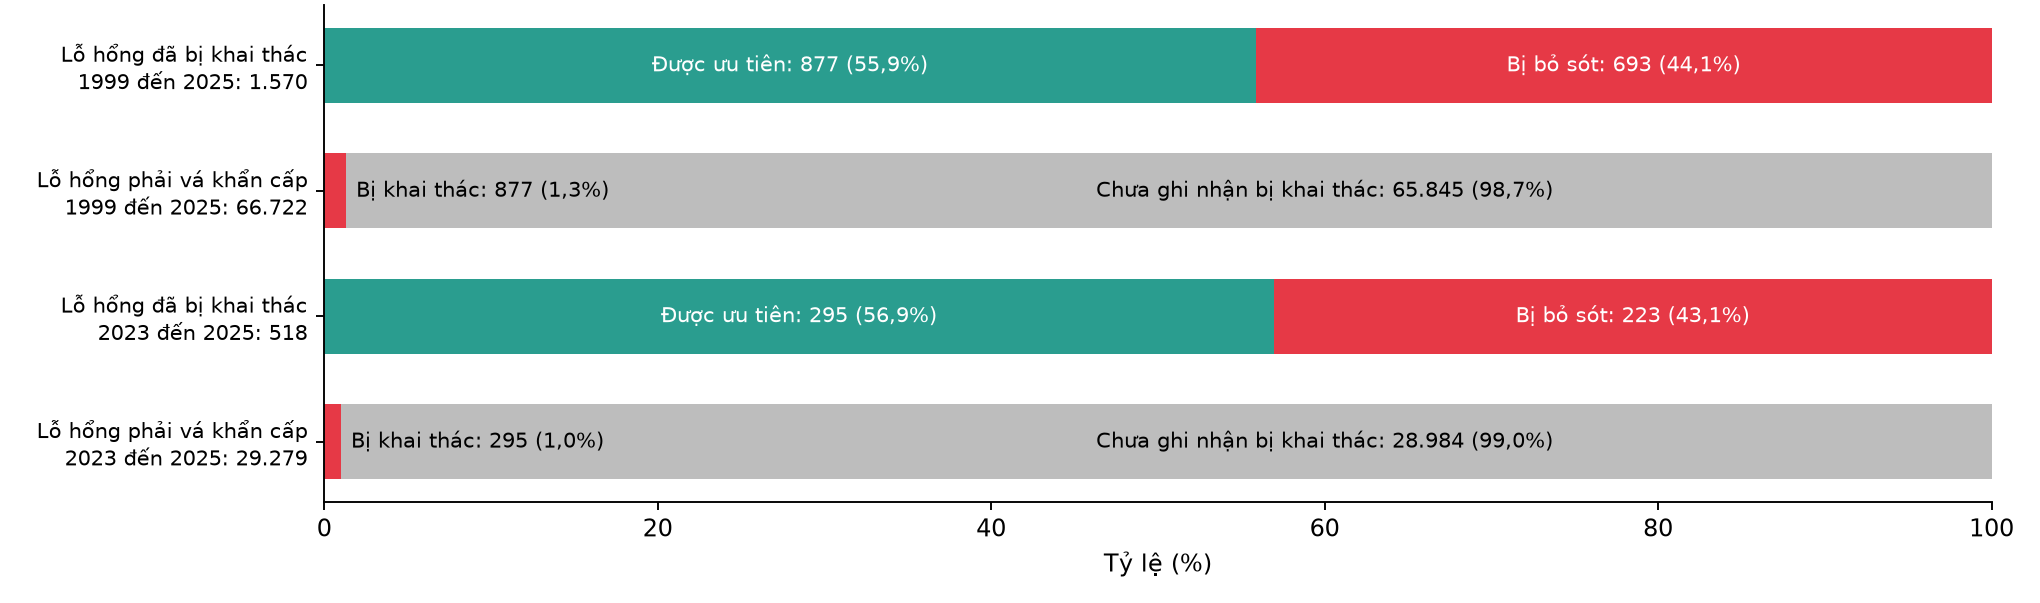
\includegraphics[width=0.85\textwidth]{nguong_hai_loi.png}
\caption{Ngưỡng CVSS 8,0 bỏ sót khoảng 44\% lỗ hổng bị khai thác, trong khi khoảng 99\% lỗ hổng
phải vá khẩn cấp chưa được ghi nhận là bị khai thác.}\label{fig:hailoi}
\end{figure*}

Đổi ngưỡng không giải quyết được vấn đề (Bảng~\ref{tab:nguong}): ngưỡng 7,0 bỏ sót 11,40\% nhưng
phải vá 54,33\% số lỗ hổng; ngưỡng 9,0 bỏ sót 65,99\%. CVSS có khả năng phân biệt ở mức độ nhất định: xác suất
vào KEV tăng từ 0,17\% (CVSS 4,0 đến 6,9) lên 1,54\% (CVSS 9,0 đến 10), tức khoảng 9 lần; nhưng tỷ lệ nền
quá thấp, nên ngay cả nhóm điểm cao nhất cũng chỉ có khoảng 1 trong 65 lỗ hổng bị khai thác. Tỷ lệ
lỗ hổng KEV có CVSS dưới 8,0 dao động từ 32\% đến 57\% qua các năm từ 2010 đến 2025 và không có xu hướng rõ rệt.
Trong 693 lỗ hổng bị bỏ sót, Microsoft chiếm 35,8\%, Apple 7,8\%, Cisco 5,9\%: phần bị bỏ sót tập
trung ở các nhà cung cấp lớn.

\begin{table}[htbp]
\caption{So sánh các ngưỡng CVSS, 1999 đến 2025}\label{tab:nguong}
\centering
\begin{tabular}{lccc}
\toprule
Ngưỡng & Phải vá & Bỏ sót KEV & Độ chính xác \\
\midrule
CVSS $\ge 7{,}0$ & 54,33\% & 11,40\% & 1,06\% \\
CVSS $\ge 8{,}0$ & 27,75\% & 44,14\% & 1,31\% \\
CVSS $\ge 9{,}0$ & 14,43\% & 65,99\% & 1,54\% \\
\bottomrule
\end{tabular}
\end{table}

\subsection{Độ nhạy của quy tắc CSA}\label{sec:donhay}
Bảng~\ref{tab:donhay} lặp lại thống kê mô tả của TN1 với năm cách đọc khuyến nghị. Với cách đọc Q0, kết quả trùng với TN1: 877
lỗ hổng KEV được ưu tiên và 693 lỗ hổng bị bỏ sót.

\begin{table*}[t]
\caption{Năm cách đọc quy tắc CSA, thống kê mô tả 1999 đến 2025; Q2 và Q4 chỉ xét lỗ hổng có vector
\texttt{AV:N}, trong đó có 1.143 lỗ hổng KEV}\label{tab:donhay}
\centering
\begin{tabular}{lrccccc}
\toprule
Cách đọc & Phạm vi & Phải vá & Bắt được KEV & Bỏ sót KEV & Độ chính xác & Vá cho 1 ca \\
\midrule
Q0. CVSS $\ge 8{,}0$ & 240.409 & 27,75\% & 55,86\% & 44,14\% & 1,31\% & 76,1 \\
Q1. CVSS $> 8{,}0$ & 240.409 & 27,35\% & 55,29\% & 44,71\% & 1,32\% & 75,8 \\
Q2. Q0, chỉ \texttt{AV:N} & 174.803 & 35,97\% & 73,75\% & 26,25\% & 1,34\% & 74,6 \\
Q3. Q0 hoặc có PoC & 240.409 & 29,01\% & 66,88\% & 33,12\% & 1,51\% & 66,4 \\
Q4. Q3, chỉ \texttt{AV:N} & 174.803 & 37,11\% & 79,27\% & 20,73\% & 1,40\% & 71,6 \\
\bottomrule
\end{tabular}
\end{table*}

Có ba điểm rút ra. Thứ nhất, đọc ``above 8.0'' theo nghĩa chặt gần như không làm thay đổi kết quả: chỉ 968
lỗ hổng có CVSS đúng bằng 8,0, trong đó 9 lỗ hổng nằm trong KEV. Thứ hai, tỷ lệ bỏ sót phụ thuộc
mạnh vào cách đọc: 72,80\% lỗ hổng KEV khai thác được qua mạng, và trong phạm vi này quy tắc chỉ bỏ
sót 26,25\%; thêm điều kiện có PoC công khai, cách đọc sát nhất (Q4) chỉ bỏ sót 20,73\%. Con số
44\% của TN1 vì vậy là cận trên, ứng với cách đọc đơn giản nhất. Thứ ba, vấn đề vá thừa không đổi:
ở mọi cách đọc, nhóm phải vá chiếm 27\% đến 37\% phạm vi xét và chỉ 1,31\% đến 1,51\% trong đó bị khai thác,
tức phải vá 66 đến 76 lỗ hổng mới gặp một lỗ hổng bị khai thác.

Kiểm thử ngược tại ba ngày đánh giá (Bảng~\ref{tab:donhay2}) cho cùng kết luận. Mọi cách đọc đều
có hiệu suất 1,7 đến 2,3 lần so với chọn ngẫu nhiên, rất xa mức 22,6 đến 27,9 lần của ngưỡng $S \ge 70$ ở cùng
ba ngày (Bảng~\ref{tab:khancap}). Khi vá cùng khối lượng với từng cách đọc, $S$ bắt được bằng hoặc
nhiều hơn quy tắc ở 13/15 trường hợp. Hai trường hợp ngược lại đều ở năm 2024 với cách đọc có PoC
(Q3: 55 so với 49; Q4: 51 so với 46). PoC công khai vì vậy là một tín hiệu có giá trị mà $S$ chưa
dùng, phù hợp với kết quả của Allodi và Massacci~\cite{allodi2014}.

\begin{table}[htbp]
\caption{Kiểm thử ngược năm cách đọc quy tắc CSA tại 31/12/2023, 31/12/2024 và 30/06/2025; HS:
hiệu suất (số lần so với chọn ngẫu nhiên); cột cuối là số lỗ hổng vào KEV mà $S$ bắt được nhiều
hơn quy tắc khi vá cùng khối lượng, lần lượt ở ba ngày}\label{tab:donhay2}
\centering
\footnotesize
\setlength{\tabcolsep}{2.5pt}
\begin{tabular}{lcccc}
\toprule
Cách đọc & Khối lượng vá & HS quy tắc & HS $S$ & $S$ hơn quy tắc \\
\midrule
Q0 & 27,7 đến 29,0\% & 2,1 & 2,1 đến 2,9 & $+13$; $0$; $+11$ \\
Q1 & 27,3 đến 28,7\% & 2,1 & 2,2 đến 2,9 & $+13$; $+2$; $+13$ \\
Q2 & 36,1 đến 37,7\% & 1,7 đến 1,9 & 1,9 đến 2,4 & $+14$; $+1$; $+5$ \\
Q3 & 29,1 đến 30,8\% & 2,2 đến 2,3 & 2,1 đến 2,7 & $+9$; $-6$; $+7$ \\
Q4 & 37,3 đến 39,4\% & 1,8 đến 2,0 & 1,8 đến 2,3 & $+11$; $-5$; $+3$ \\
\bottomrule
\end{tabular}
\end{table}

\subsection{Điểm S phân biệt được lỗ hổng sắp bị khai thác}
Ngày 30/06/2025 có 209.623 lỗ hổng chưa có trong KEV, chỉ 91 (0,043\%) vào KEV trong 12 tháng sau.
Tỷ lệ vào KEV tăng theo mức điểm (Bảng~\ref{tab:mucS}); các mức từ 70 có tỷ lệ từ 1,16\% đến 1,29\%, gấp 27 đến 30 lần mức trung bình. Xu hướng chung này lặp lại ở cả ba ngày (Hình~\ref{fig:mucS}), dù từng mức
dao động do số lỗ hổng vào KEV ít.

\begin{table}[htbp]
\caption{Tỷ lệ vào KEV trong 12 tháng theo mức $S$, ngày 30/06/2025}\label{tab:mucS}
\centering
\begin{tabular}{lrrrr}
\toprule
Mức $S$ & Số lỗ hổng & Vào KEV & Tỷ lệ & Gấp TB \\
\midrule
0 đến 10   & 100.819 & 11 & 0,011\% & 0,3 \\
10 đến 20  & 72.627  & 20 & 0,028\% & 0,6 \\
20 đến 30  & 17.999  & 3  & 0,017\% & 0,4 \\
30 đến 40  & 7.541   & 7  & 0,093\% & 2,1 \\
40 đến 50  & 3.769   & 4  & 0,11\%  & 2,4 \\
50 đến 60  & 2.348   & 5  & 0,21\%  & 4,9 \\
60 đến 70  & 1.717   & 7  & 0,41\%  & 9,4 \\
70 đến 80  & 1.206   & 14 & 1,16\%  & 26,7 \\
80 đến 90  & 777     & 10 & 1,29\%  & 29,6 \\
90 đến 100 & 820     & 10 & 1,22\%  & 28,1 \\
\midrule
Tổng & 209.623 & 91 & 0,043\% & 1,0 \\
\bottomrule
\end{tabular}
\end{table}

\begin{figure*}[t]
\centering
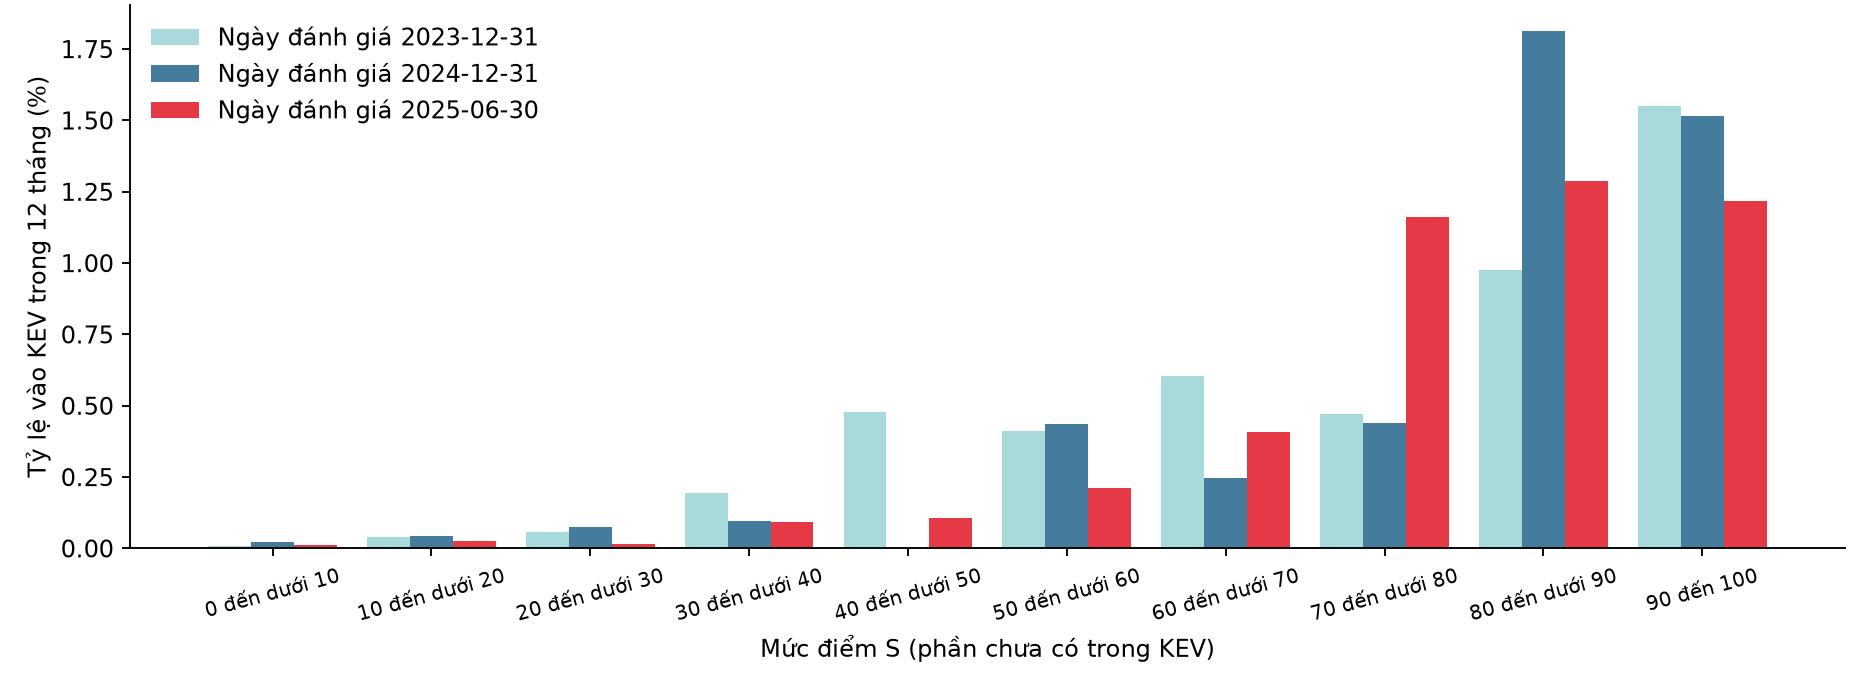
\includegraphics[width=0.85\textwidth]{S_ty_le_theo_muc.png}
\caption{Tỷ lệ vào KEV trong 12 tháng sau theo mức điểm $S$, tại ba ngày đánh giá.}\label{fig:mucS}
\end{figure*}

Bảng~\ref{tab:khancap} đặt ngưỡng $S \ge 70$ cạnh quy tắc CSA. Ngày 30/06/2025, vá mọi lỗ hổng có
$S \ge 70$ là vá 2.803 lỗ hổng (1,34\%), bắt 34/91 (37,36\%), tức 82 lỗ hổng phải vá cho mỗi lỗ hổng
bắt được; quy tắc CSA vá 58.133 lỗ hổng (27,73\%), bắt 54/91, tức 1.076 lỗ hổng cho mỗi lỗ hổng bắt
được. Quy tắc CSA bắt nhiều hơn vì vá nhiều gấp khoảng 20 lần. Tính theo hiệu suất, ngưỡng $S \ge 70$ gấp 22,6 đến 27,9 lần so với chọn ngẫu nhiên, quy tắc CSA chỉ gấp 2,1 lần, ổn định ở cả ba ngày; TN6 xác nhận
kết quả này ở 11 ngày (Mục~\ref{sec:ondinh}). Khi tính cả các lỗ hổng đã có trong KEV (theo quy tắc ở Mục~\ref{sec:giaiphap}), nhóm vá khẩn cấp chỉ chiếm 1,44 đến 1,98\%
số lỗ hổng có CVSS 3.x.

\begin{table}[htbp]
\caption{Ngưỡng $S \ge 70$ và quy tắc CSA trên phần chưa có trong KEV, tại ba ngày đánh giá; HS:
hiệu suất (số lần so với chọn ngẫu nhiên); nhóm khẩn cấp gồm thêm mọi lỗ hổng đã có trong
KEV}\label{tab:khancap}
\centering
\small
\setlength{\tabcolsep}{3pt}
\begin{tabular}{lccccc}
\toprule
 & \multicolumn{3}{c}{Ngưỡng $S \ge 70$} & \multicolumn{2}{c}{Quy tắc CSA} \\
\cmidrule(lr){2-4}\cmidrule(lr){5-6}
Ngày & Bắt được & HS & Khẩn cấp & Khối lượng & HS \\
\midrule
31/12/2023 & 14/61 & 22,6 & 1,72\% & 28,98\% & 2,1 \\
31/12/2024 & 16/80 & 25,5 & 1,44\% & 28,20\% & 2,1 \\
30/06/2025 & 34/91 & 27,9 & 1,98\% & 27,73\% & 2,1 \\
\bottomrule
\end{tabular}
\end{table}

Khi cố định cùng khối lượng vá (Bảng~\ref{tab:cungkl}), vá 1\% hoặc 5\% thì $S$ bắt được nhiều gấp
2,7 đến 8,9 lần CVSS ở cả ba ngày, khoảng tin cậy 95\% của chênh lệch đều trên 0. So với EPSS, chênh
lệch nhỏ và đổi chiều: bằng nhau ở 1\% và 5\% năm 2023 và ở 1\% năm 2024; $S$ kém 2 ca ở 5\% năm
2024, kém 5 ca ở 1\% và 1 ca ở 5\% năm 2025; ở khối lượng của quy tắc CSA, $S$ bằng hoặc hơn EPSS
ở cả ba ngày. Hình~\ref{fig:batduoc} cho thấy đường của $S$ và EPSS gần trùng nhau ở phần vá ít.

\begin{table}[htbp]
\caption{Số lỗ hổng vào KEV bắt được khi vá cùng số lượng}\label{tab:cungkl}
\centering
\setlength{\tabcolsep}{4pt}
\begin{tabular}{llrccc}
\toprule
Ngày & Vá & Số vá & CVSS & EPSS & $S$ \\
\midrule
31/12/2023 & 1\%    & 1.473  & 2,0/61  & 14/61 & 14/61 \\
           & 5\%    & 7.365  & 8,9/61  & 30/61 & 30/61 \\
           & như CSA & 42.685 & 38/61  & 49/61 & 51/61 \\
31/12/2024 & 1\%    & 1.867  & 2,0/80  & 18/80 & 18/80 \\
           & 5\%    & 9.337  & 9,7/80  & 28/80 & 26/80 \\
           & như CSA & 52.662 & 48/80  & 45/80 & 48/80 \\
30/06/2025 & 1\%    & 2.096  & 4,8/91  & 30/91 & 25/91 \\
           & 5\%    & 10.481 & 11,3/91 & 51/91 & 50/91 \\
           & như CSA & 58.133 & 54/91  & 65/91 & 65/91 \\
\bottomrule
\end{tabular}
\end{table}

\begin{figure*}[t]
\centering
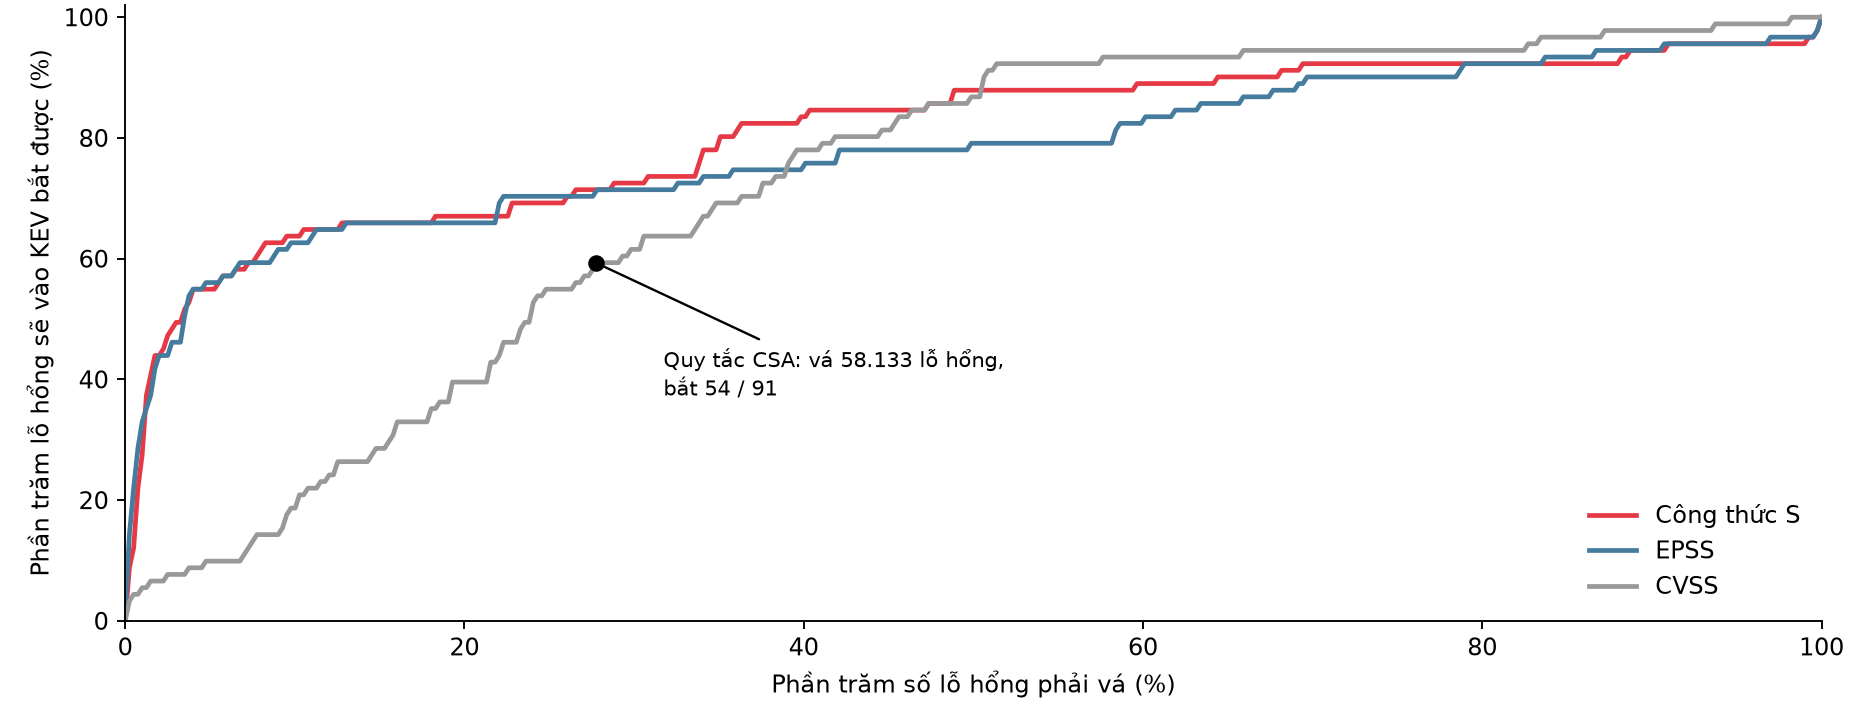
\includegraphics[width=0.85\textwidth]{S_duong_bat_duoc.png}
\caption{Đường bắt được ngày 30/06/2025: phần trăm lỗ hổng sẽ vào KEV bắt được theo phần trăm lỗ
hổng phải vá. Chấm đen là quy tắc CSA.}\label{fig:batduoc}
\end{figure*}

\subsection{Độ ổn định qua 11 ngày đánh giá và theo số mũ}\label{sec:ondinh}
TN6 lặp lại thiết kế của TN2 tại 11 ngày cuối quý. Ba ngày trùng với TN2 cho đúng cùng số lỗ hổng,
số lỗ hổng vào KEV và số lỗ hổng $S$ bắt được. Tổng cộng có 776 lượt lỗ hổng vào KEV trong 12 tháng
sau các ngày đánh giá, từ 39 đến 91 mỗi ngày.

Bảng~\ref{tab:ondinh} và Hình~\ref{fig:ondinh} cho thấy ba kết quả. Thứ nhất, ngưỡng $S \ge 70$ ổn
định: ở cả 11 ngày, nhóm này chỉ chiếm 0,78\% đến 1,40\% số lỗ hổng chưa có trong KEV nhưng bắt được 14,1\% đến 44,2\% số lỗ hổng sẽ vào KEV, tức hiệu suất 15,9 đến 34,2 lần so với chọn ngẫu nhiên; quy tắc CSA chỉ đạt 1,7 đến 2,3 lần. Thứ hai, $S$ không kém CVSS ở bất kỳ ngày nào và ở bất kỳ khối lượng vá nào, kể cả
ba ngày có cửa sổ theo dõi không chồng nhau. So với EPSS, $S$ không kém ở 6 đến 9 trong 11 ngày tùy
khối lượng vá. Thứ ba, trên tập lỗ hổng tồn đọng này, $S$ và EPSS gần
như ngang nhau ở mọi khối lượng: khi gộp 11 ngày, chênh lệch không quá 2 điểm phần trăm. Lợi thế của $S$ so với EPSS khi vá nhiều chỉ thấy rõ ở dữ liệu lỗ hổng mới công bố của TN4 (Bảng~\ref{tab:a1}).

\begin{table}[htbp]
\caption{Tỷ lệ lỗ hổng vào KEV trong 12 tháng sau mà mỗi cách bắt được khi vá cùng số lượng, gộp 11 ngày cuối quý
(776 lỗ hổng) và riêng ba ngày có cửa sổ theo dõi không chồng nhau (201 lỗ hổng)}\label{tab:ondinh}
\centering
\setlength{\tabcolsep}{5pt}
\begin{tabular}{llccc}
\toprule
Nhóm ngày & Khối lượng & CVSS & EPSS & $S$ \\
\midrule
11 ngày & 1\%     & 3,7\%  & 25,9\% & 24,9\% \\
        & 5\%     & 13,8\% & 44,2\% & 43,9\% \\
        & 10\%    & 26,4\% & 53,0\% & 53,5\% \\
        & 25\%    & 54,1\% & 66,7\% & 67,0\% \\
        & như CSA & 59,3\% & 68,8\% & 70,8\% \\
\midrule
3 ngày  & 1\%     & 3,0\%  & 28,4\% & 25,9\% \\
không   & 5\%     & 13,6\% & 43,8\% & 44,3\% \\
chồng   & 10\%    & 26,9\% & 53,2\% & 55,2\% \\
nhau    & 25\%    & 52,9\% & 67,7\% & 68,2\% \\
        & như CSA & 58,2\% & 69,2\% & 70,1\% \\
\bottomrule
\end{tabular}
\end{table}

\begin{figure*}[t]
\centering
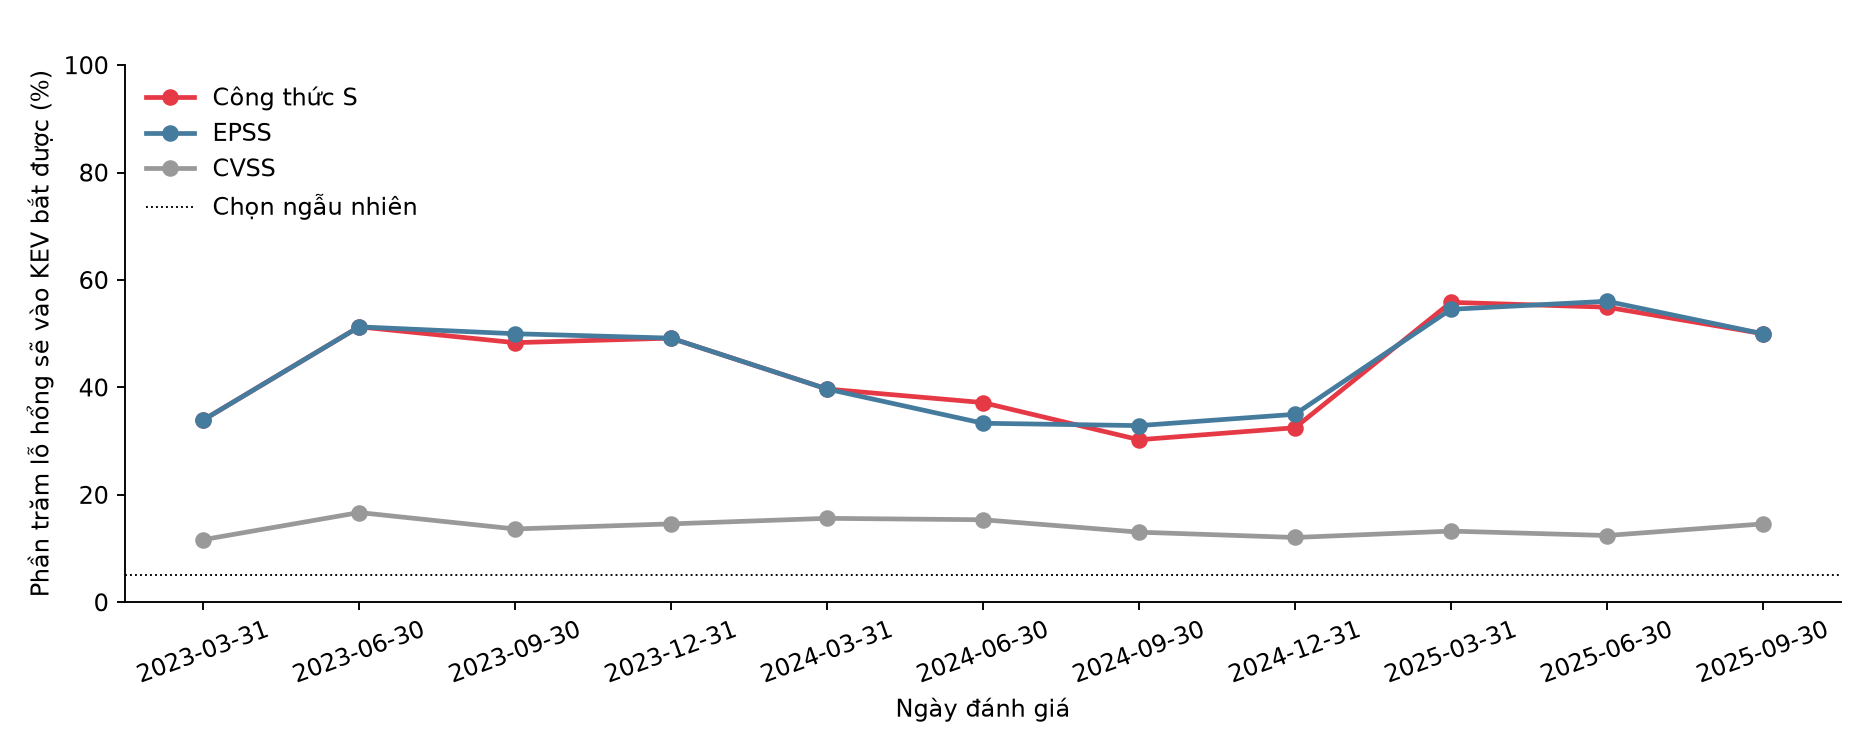
\includegraphics[width=0.85\textwidth]{nhieu_ngay_va_5.png}
\caption{Vá 5\% số lỗ hổng chưa có trong KEV tại 11 ngày đánh giá: phần trăm lỗ hổng vào KEV trong 12 tháng sau mà mỗi cách bắt được. Đường chấm là chọn ngẫu nhiên.}\label{fig:ondinh}
\end{figure*}

Ngưỡng $S \ge 70$ cũng cho thấy ảnh hưởng của phiên bản EPSS: khối lượng của nhóm này giảm dần từ
1,17\% xuống 0,78\% trong thời gian dùng mô hình v2023.03.01 (31/03/2023 đến 31/12/2024), rồi tăng
lên 1,30\% đến 1,40\% khi FIRST chuyển sang mô hình v2025.03.14.

Bảng~\ref{tab:somu} quét số mũ của EPSS trên cả 11 ngày. Mọi số mũ từ 0,2 đến 1,0 cho kết quả gần
như nhau (trung bình của bốn khối lượng từ 47,1\% đến 47,8\%). Số mũ 0,1 kém hơn khi vá ít (22,2\% so với 24,9\%
khi vá 1\%) nhưng tốt nhất khi vá 25\% (69,3\%), vì số mũ càng nhỏ thì CVSS càng có trọng lượng. Không
có số mũ tối ưu chung; 0,3 nằm trong nhóm cho kết quả tốt, nên kết luận của báo cáo không phụ thuộc
vào lựa chọn này.

\begin{table}[htbp]
\caption{Quét số mũ của EPSS trong $S$, gộp 11 ngày: tỷ lệ lỗ hổng vào KEV bắt được theo khối lượng vá}\label{tab:somu}
\centering
\setlength{\tabcolsep}{4pt}
\begin{tabular}{cccccc}
\toprule
Số mũ & 1\% & 5\% & 10\% & 25\% & Trung bình \\
\midrule
0,1 & 22,2\% & 41,1\% & 50,6\% & 69,3\% & 45,8\% \\
0,2 & 24,7\% & 43,8\% & 52,2\% & 67,5\% & 47,1\% \\
0,3 & 24,9\% & 43,9\% & 53,5\% & 67,0\% & 47,3\% \\
0,5 & 25,9\% & 44,3\% & 54,1\% & 66,9\% & 47,8\% \\
0,7 & 25,8\% & 44,3\% & 54,3\% & 66,6\% & 47,7\% \\
1,0 & 25,8\% & 44,2\% & 54,0\% & 66,9\% & 47,7\% \\
\bottomrule
\end{tabular}
\end{table}

\subsection{Điểm trước khi được CISA xác nhận}
Trong 836 lỗ hổng vào KEV từ 01/04/2023, 227 (27,15\%) chưa có EPSS một ngày trước khi vào KEV;
226 trong số đó công bố cùng ngày hoặc một ngày trước. Đây là zero-day: không công thức nào chấm
được điểm trước, chỉ quy tắc KEV đưa chúng vào nhóm vá khẩn cấp ngay khi được xác nhận.

Với 609 lỗ hổng còn lại, EPSS một ngày trước khi vào KEV thường rất thấp: trung vị chỉ 0,0038. Vì
vậy $S$ trước khi vào KEV thấp hơn nhiều $S$ khi vào KEV (Hình~\ref{fig:truockev}); điểm khi vào
KEV bằng $\mathit{CVSS} \times 10$ theo định nghĩa, nên khoảng cách giữa hai điểm phản ánh chính
EPSS chứ không phải một kết quả riêng. Bảng~\ref{tab:tuoi} chia theo tuổi lỗ hổng: với lỗ hổng công bố không quá 30 ngày trước khi vào KEV, trung vị EPSS chỉ 0,0009 và chỉ 4,46\% có $S \ge 70$;
với lỗ hổng công bố hơn 1 năm, tỷ lệ này là 35,98\%. Trong 108 lỗ hổng có $S \ge 70$ một ngày
trước khi vào KEV, 68 (62,96\%) đã công bố hơn 1 năm. Công thức hữu ích với lỗ hổng cũ còn tồn
đọng, nhưng gần như không cảnh báo trước được lỗ hổng mới công bố, đúng nhóm mà CSA lo ngại.

\begin{table}[htbp]
\caption{Điểm một ngày trước khi vào KEV theo thời gian từ ngày công bố đến ngày vào KEV}\label{tab:tuoi}
\centering
\footnotesize
\setlength{\tabcolsep}{3pt}
\begin{tabular}{L{2.4cm}cccc}
\toprule
Nhóm lỗ hổng KEV & Số & EPSS trung vị & $S \ge 70$ & $S \ge 50$ \\
\midrule
Chưa có EPSS (zero-day) & 227 & không có & không có & không có \\
Công bố $\le 30$ ngày trước & 224 & 0,0009 & 4,46\% & 7,14\% \\
Công bố từ 31 đến 365 ngày trước & 196 & 0,0039 & 15,31\% & 22,96\% \\
Công bố hơn 1 năm trước & 189 & 0,0709 & 35,98\% & 45,50\% \\
\midrule
Tất cả có EPSS & 609 & 0,0038 & 17,73\% & 24,14\% \\
\bottomrule
\end{tabular}
\end{table}

\begin{figure*}[t]
\centering
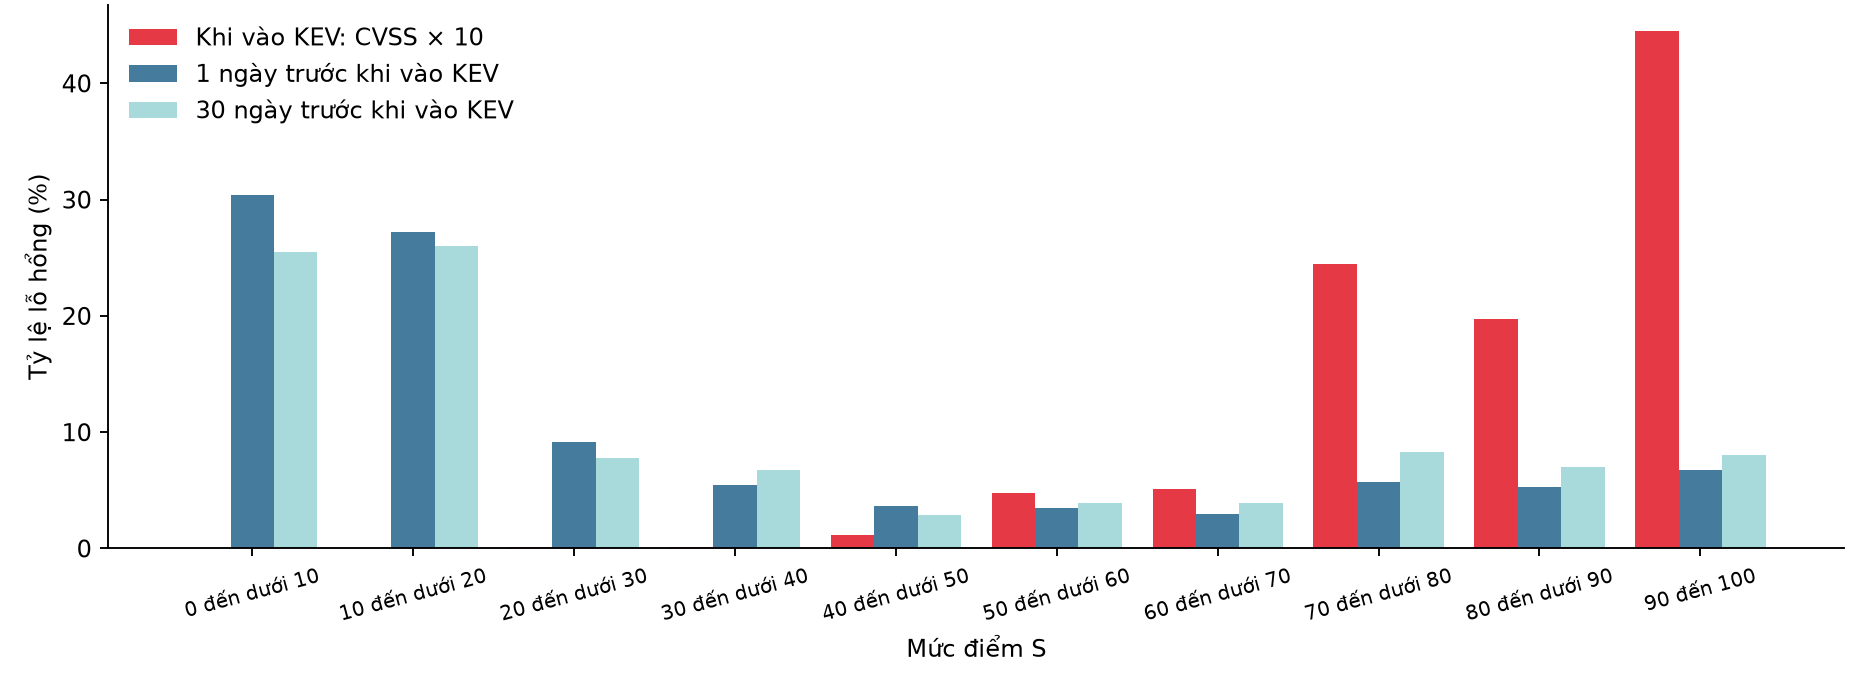
\includegraphics[width=0.85\textwidth]{truoc_kev_muc_diem.png}
\caption{Mức điểm $S$ của 609 lỗ hổng KEV: 30 ngày trước, 1 ngày trước và khi vào KEV (khi vào KEV,
$S = \mathit{CVSS} \times 10$ theo định nghĩa).}\label{fig:truockev}
\end{figure*}

Xét theo hiệu suất (Bảng~\ref{tab:truockev}), mức $S \ge 70$ một ngày trước khi vào KEV chiếm 1,34\%
khối lượng vá nhưng chứa 17,73\% lỗ hổng sắp vào KEV, gấp khoảng 13 lần ngẫu nhiên; quy tắc CSA chỉ
gấp 2,3 lần. Con số này chỉ là ước lượng: khối lượng vá lấy từ ngày 30/06/2025, còn các lỗ hổng vào
KEV rải rác từ 2023 đến 2026. Kết quả sạch hơn là của TN2 (Bảng~\ref{tab:khancap}).

\begin{table}[htbp]
\caption{Trước khi vào KEV: tỷ lệ lỗ hổng sắp vào KEV được ưu tiên}\label{tab:truockev}
\centering
\begin{tabular}{lccc}
\toprule
Cách ưu tiên & Chứa được & Khối lượng & Gấp NN \\
\midrule
CSA: CVSS $\ge 8{,}0$ & 64,20\% & 27,73\% & 2,3 \\
$S \ge 30$ & 33,17\% & 8,67\% & 3,8 \\
$S \ge 50$ & 24,14\% & 3,28\% & 7,4 \\
$S \ge 70$ & 17,73\% & 1,34\% & 13,3 \\
\bottomrule
\multicolumn{4}{l}{\footnotesize $S$ tính bằng EPSS 1 ngày trước khi vào KEV; NN: ngẫu nhiên.}
\end{tabular}
\end{table}

\subsection{Tình huống điển hình: CVSS nói thấp, thực tế nói cao}\label{sec:tinhhuong}

Phần này trình bày các tình huống cụ thể dưới dạng ví dụ minh họa thực tế (\emph{case in point}), lấy từ
dữ liệu của chúng tôi (thực nghiệm 7). Để tránh chọn ví dụ có lợi, các tình huống được chọn theo \emph{tiêu chí
đặt trước}, và báo cáo cả số trường hợp không đạt:
\begin{itemize}
\item \textbf{Công thức bắt trước, quy tắc CSA bỏ qua:} lỗ hổng vào KEV từ 01/04/2023, có CVSS dưới 8,0 (quy
tắc CSA không bao giờ ưu tiên), và có $S \ge 50$ tại thời điểm 30 ngày trước khi vào KEV. Ngày 30/06/2025, chỉ
6.868 / 209.623 = 3,28\% lỗ hổng chưa có trong KEV đạt $S \ge 50$.
\item \textbf{Ba tình huống vẽ lịch sử điểm theo tháng}, chọn theo quy tắc: CVSS thấp nhất, báo trước lâu nhất,
thời gian từ công bố đến khi vào KEV ngắn nhất.
\item \textbf{Quy tắc CSA vá thừa:} lỗ hổng CVSS $\ge 9{,}0$ chưa có trong KEV tại ngày 30/06/2025.
\item \textbf{Trường hợp công thức không bắt được}, gồm ví dụ CVE-2025-13956 do CrowdSec công bố~\cite{crowdsec2026}.
\end{itemize}

\subsubsection{Tình huống 1: CVSS nói 5,3, công thức nói 52 (CVE-2021-26086, Atlassian Jira)}
\begin{itemize}
\item Lỗ hổng của Jira Server và Data Center, công bố 16/08/2021, CVSS 5,3 (mức trung bình).
\item Quy tắc CSA: không bao giờ ưu tiên lỗ hổng này.
\item Công thức $S$: điểm tăng dần theo EPSS, từ 11 (09/2021) lên 45 (03/2022). $S$ đạt 50 lần đầu vào
03/2023 (đúng tháng EPSS đổi mô hình), sau đó có 5 tháng rơi lại dưới 50; chuỗi tháng liên tục có $S \ge 50$ bắt đầu khoảng
8 tháng trước khi vào KEV.
\item CISA đưa vào KEV ngày 12/11/2024. Ba mươi ngày trước đó, EPSS đã là 0,8549 và $S = 50{,}6$.
\item Kết quả: công thức đưa lỗ hổng vào nhóm ưu tiên cao ($S \ge 50$) khoảng 8 đến 19 tháng trước khi CISA
xác nhận, tùy tính từ chuỗi liên tục hay từ lần đầu. Quy tắc CVSS để nó nằm trong danh sách tồn đọng suốt thời
gian đó.
\item Giới hạn: với CVSS 5,3, $S$ tối đa chỉ 53, nên lỗ hổng này không bao giờ vào nhóm vá khẩn cấp
($S \ge 70$) trước khi vào KEV. Chỉ khi lỗ hổng vào KEV, quy tắc KEV mới đưa nó vào nhóm vá khẩn cấp.
\end{itemize}

\subsubsection{Tình huống 2: từ 7 lên 62 điểm trong hai tháng (CVE-2023-32315, Ignite Realtime Openfire)}
Bảng~\ref{tab:openfire} cho thấy dạng ``chuyển pha'': lỗ hổng chuyển nhanh từ trạng thái bình thường sang trạng thái bị khai thác.
Công thức tính lại điểm hằng ngày theo EPSS nên nhận ra thay đổi gần một tháng trước khi CISA xác nhận, dù điểm
62 mới chỉ ở mức ưu tiên cao, chưa tới ngưỡng vá khẩn cấp 70. Khi lỗ hổng vào KEV, thành phần KEV đẩy điểm lên mức
cao nhất của nó. Điểm CVSS vẫn là 7,5 như ngày công bố.

\begin{table}[t]
\centering
\caption{Điểm $S$ theo tháng của CVE-2023-32315 (Openfire, CVSS 7,5)}\label{tab:openfire}
\footnotesize
\begin{tabular}{lcc}
\toprule
Ngày & Điểm $S$ & Quy tắc CSA \\
\midrule
31/05/2023 (công bố 26/05/2023) & 7 & Không ưu tiên \\
30/06/2023 & 34 & Không ưu tiên \\
31/07/2023 & 62 & Không ưu tiên \\
24/08/2023: vào KEV & 75 ($\mathit{CVSS} \times 10$) & Không ưu tiên \\
\bottomrule
\end{tabular}
\end{table}

\subsubsection{Tình huống 3: CISA xác nhận sau công thức hơn 4 năm (CVE-2015-5477, ISC BIND)}
\begin{itemize}
\item Lỗ hổng BIND, công bố 29/07/2015, CVSS 7,5.
\item Công thức $S$: điểm ở mức khoảng 73 liên tục từ 02/2022, thuộc nhóm khoảng 1,3\% lỗ hổng có điểm cao nhất.
\item CISA đưa vào KEV ngày 08/10/2026, tức công thức báo trước khoảng 55 tháng.
\item Quy tắc CSA: không ưu tiên ở bất kỳ thời điểm nào.
\end{itemize}
Hình~\ref{fig:tinhhuong} vẽ điểm theo tháng của ba tình huống.

\begin{figure*}[t]
\centering
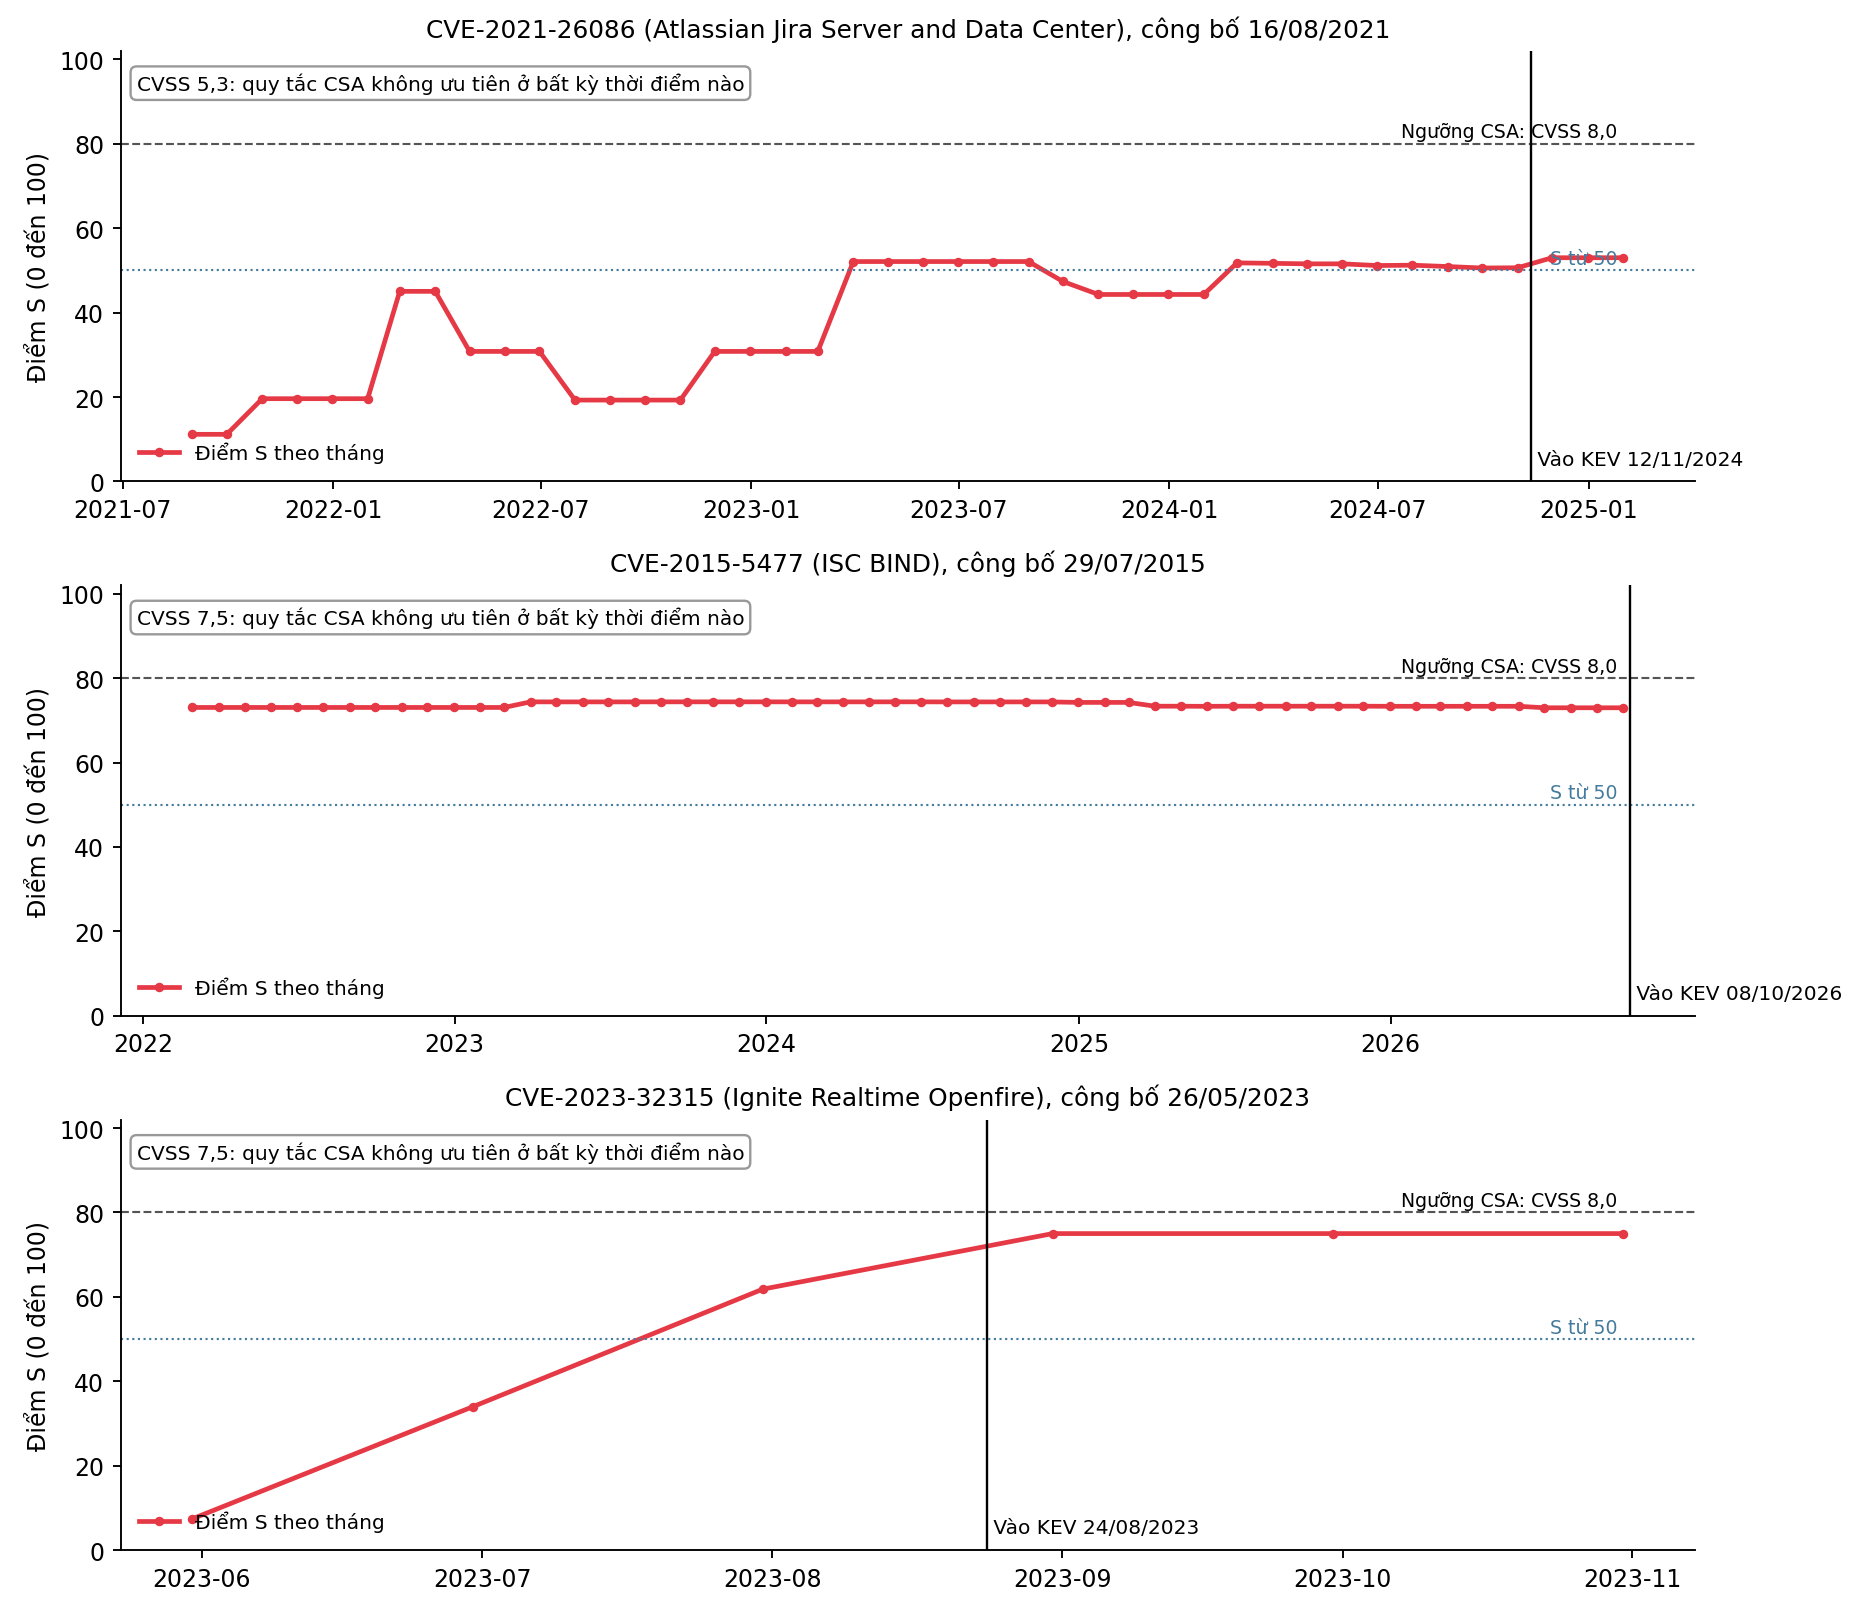
\includegraphics[width=0.7\textwidth]{tinh_huong_lich_su_diem.png}
\caption{Điểm $S$ theo tháng của ba tình huống. Đường nét đứt ở 80 ứng với ngưỡng CVSS 8,0 của CSA
(nhân 10), đường chấm ở 50 là ngưỡng ưu tiên cao, đường thẳng đứng là ngày vào KEV; cả ba có CVSS dưới
8,0 nên quy tắc CSA không ưu tiên ở bất kỳ thời điểm nào.}\label{fig:tinhhuong}
\end{figure*}

\subsubsection{Tổng hợp theo tiêu chí}
Bảng~\ref{tab:tonghopth} tổng hợp 328 lỗ hổng vào KEV từ 01/04/2023 có CVSS dưới 8,0. Hai cách tính thời gian báo trước (thực
nghiệm 7) khác nhau ở 5 lỗ hổng mà điểm rơi lại dưới 50 sau lần đầu vượt ngưỡng (CVE-2021-22555, CVE-2020-9715,
CVE-2021-26086, CVE-2021-41277, CVE-2022-43769); cách tính liên tục $B_{\text{lt}}$ sát hơn với việc tổ chức thực
sự giữ lỗ hổng trong nhóm ưu tiên. Với 19 lỗ hổng còn lại, hai cách cho cùng kết quả. Ví dụ CVE-2021-41277: $S$
đạt 50 lần đầu ngày 31/03/2023, rơi xuống 31,9 đến 39,3 từ 09/2023 đến 01/2024, trở lại 74,0 ngày 29/02/2024 và
giữ mức đó tới khi vào KEV ngày 12/11/2024, nên $B_{\text{lt}} = 257 / 30{,}44 \approx 8$ tháng thay vì
$B = 592 / 30{,}44 \approx 19$ tháng. Bảng~\ref{tab:ds24} liệt kê đầy đủ 24 lỗ hổng mà công thức bắt trước;
Bảng~\ref{tab:baotruoc} cho thời gian báo trước của từng lỗ hổng.

\begin{table}[t]
\centering
\caption{Tổng hợp theo tiêu chí: 328 lỗ hổng vào KEV từ 01/04/2023 có CVSS dưới 8,0, quy tắc CSA bỏ qua toàn bộ}\label{tab:tonghopth}
\footnotesize
\begin{tabular}{>{\raggedright\arraybackslash}p{4.6cm}>{\raggedright\arraybackslash}p{3.4cm}}
\toprule
Hạng mục & Số lượng \\
\midrule
Có điểm EPSS 30 ngày trước khi vào KEV & 156 / 328 = 47,56\% \\
$S \ge 50$ tại thời điểm 30 ngày trước khi vào KEV (công thức bắt trước) & 24 / 156 = 15,38\% (trên cả 328: 24 / 328 = 7,32\%) \\
$S \ge 70$ tại thời điểm 30 ngày trước khi vào KEV (ngưỡng vá khẩn cấp) & 14 / 156 = 8,97\% (trên cả 328: 14 / 328 = 4,27\%) \\
Trong 24 lỗ hổng bắt trước, báo trước từ 12 tháng trở lên, tính từ lần đầu $S \ge 50$ & 18 / 24 = 75,00\% (trung vị 19,4 tháng) \\
Như trên, tính từ đầu chuỗi tháng liên tục có $S \ge 50$ & 15 / 24 = 62,50\% (trung vị 14,3 tháng) \\
$S < 30$ tại thời điểm 30 ngày trước khi vào KEV (công thức không bắt trước) & 119 / 156 = 76,28\% \\
\bottomrule
\end{tabular}
\end{table}

\begin{table*}[t]
\centering
\caption{Danh sách đầy đủ 24 lỗ hổng mà công thức bắt trước còn quy tắc CSA bỏ qua: CVSS dưới 8,0 và $S \ge 50$ tại thời điểm 30 ngày trước khi vào KEV, sắp xếp giảm dần theo $S_{-30}$. EPSS$_{-30}$, $S_{-30}$: EPSS và $S$ 30 ngày trước khi vào KEV; $S_{\mathrm{KEV}}$: $S$ khi vào KEV; MĐTT: đã dùng trong mã độc tống tiền theo KEV.}\label{tab:ds24}
\footnotesize
\begin{tabular}{r l >{\raggedright\arraybackslash}p{4.2cm} c c c c c c c}
\toprule
STT & Mã CVE & Sản phẩm & CVSS & Công bố & Vào KEV & EPSS$_{-30}$ & $S_{-30}$ & $S_{\mathrm{KEV}}$ & MĐTT \\
\midrule
1 & CVE-2016-6415 & Cisco IOS, IOS XR, IOS XE & 7,5 & 19/09/2016 & 19/05/2023 & 0,9727 & 74,4 & 75,0 & Chưa rõ \\
2 & CVE-2016-9079 & Mozilla Firefox, Thunderbird & 7,5 & 11/06/2018 & 22/06/2023 & 0,9719 & 74,4 & 75,0 & Chưa rõ \\
3 & CVE-2020-17519 & Apache Flink & 7,5 & 05/01/2021 & 23/05/2024 & 0,9708 & 74,3 & 75,0 & Chưa rõ \\
4 & CVE-2021-41277 & Metabase & 7,5 & 17/11/2021 & 12/11/2024 & 0,9515 & 73,9 & 75,0 & Chưa rõ \\
5 & CVE-2021-43798 & Grafana Labs Grafana & 7,5 & 07/12/2021 & 09/10/2025 & 0,9434 & 73,7 & 75,0 & Chưa rõ \\
6 & CVE-2019-5418 & Rails Ruby on Rails & 7,5 & 27/03/2019 & 07/07/2025 & 0,9423 & 73,7 & 75,0 & Chưa rõ \\
7 & CVE-2020-25078 & D-Link DCS-2530L, DCS-2670L & 7,5 & 02/09/2020 & 05/08/2025 & 0,9403 & 73,6 & 75,0 & Chưa rõ \\
8 & CVE-2021-22555 & Linux Kernel & 7,8 & 07/07/2021 & 06/10/2025 & 0,8242 & 73,6 & 78,0 & Chưa rõ \\
9 & CVE-2017-3506 & Oracle WebLogic Server & 7,4 & 24/04/2017 & 03/06/2024 & 0,9688 & 73,3 & 74,0 & Chưa rõ \\
10 & CVE-2019-9621 & Synacor Zimbra & 7,5 & 30/04/2019 & 07/07/2025 & 0,9181 & 73,1 & 75,0 & Chưa rõ \\
11 & CVE-2015-5477 & ISC BIND & 7,5 & 29/07/2015 & 08/10/2026 & 0,9128 & 73,0 & 75,0 & Chưa rõ \\
12 & CVE-2021-22054 & Omnissa Workspace ONE UEM & 7,5 & 17/12/2021 & 09/03/2026 & 0,8893 & 72,4 & 75,0 & Chưa rõ \\
13 & CVE-2024-21182 & Oracle WebLogic Server & 7,5 & 16/07/2024 & 01/06/2026 & 0,8767 & 72,1 & 75,0 & Chưa rõ \\
14 & CVE-2024-27199 & JetBrains TeamCity & 7,3 & 04/03/2024 & 20/04/2026 & 0,9449 & 71,8 & 73,0 & Có \\
15 & CVE-2021-21311 & Adminer & 7,2 & 11/02/2021 & 29/09/2025 & 0,8753 & 69,2 & 72,0 & Chưa rõ \\
16 & CVE-2020-9715 & Adobe Acrobat & 7,8 & 19/08/2020 & 13/04/2026 & 0,5621 & 65,6 & 78,0 & Chưa rõ \\
17 & CVE-2023-32315 & Ignite Realtime Openfire & 7,5 & 26/05/2023 & 24/08/2023 & 0,5255 & 61,8 & 75,0 & Chưa rõ \\
18 & CVE-2018-9276 & Paessler PRTG Network Monitor & 7,2 & 02/07/2018 & 04/02/2025 & 0,5241 & 59,3 & 72,0 & Chưa rõ \\
19 & CVE-2023-27351 & PaperCut NG/MF & 7,5 & 20/04/2023 & 20/04/2026 & 0,4475 & 58,9 & 75,0 & Có \\
20 & CVE-2022-43769 & Hitachi Vantara Pentaho BA & 7,2 & 03/04/2023 & 03/03/2025 & 0,3560 & 52,8 & 72,0 & Chưa rõ \\
21 & CVE-2023-24955 & Microsoft SharePoint Server & 7,2 & 09/05/2023 & 26/03/2024 & 0,3361 & 51,9 & 72,0 & Có \\
22 & CVE-2021-39935 & GitLab CE/EE & 7,5 & 13/12/2021 & 03/02/2026 & 0,2825 & 51,3 & 75,0 & Chưa rõ \\
23 & CVE-2021-26086 & Atlassian Jira Server, DC & 5,3 & 16/08/2021 & 12/11/2024 & 0,8549 & 50,6 & 53,0 & Chưa rõ \\
24 & CVE-2023-0386 & Linux Kernel & 7,8 & 22/03/2023 & 17/06/2025 & 0,2318 & 50,3 & 78,0 & Chưa rõ \\
\bottomrule
\end{tabular}
\end{table*}

\begin{table*}[t]
\caption{24 lỗ hổng CVSS dưới 8,0 có $S \ge 50$ 30 ngày trước khi vào KEV; $B$ và $B_{\text{lt}}$
tính bằng tháng}\label{tab:baotruoc}
\centering
\footnotesize
\setlength{\tabcolsep}{2pt}
\begin{tabular}{lccccccl@{\hspace{1em}}lccccccl}
\toprule
Mã CVE & CVSS & Lần đầu & Trở lại & Vào KEV & $B$ & $B_{\text{lt}}$ & Lần đầu đạt &
Mã CVE & CVSS & Lần đầu & Trở lại & Vào KEV & $B$ & $B_{\text{lt}}$ & Lần đầu đạt \\
\midrule
CVE-2015-5477 & 7,5 & 02/2022 & 02/2022 & 10/2026 & 55 & 55 & Đổi MH &
CVE-2016-6415 & 7,5 & 02/2022 & 02/2022 & 05/2023 & 15 & 15 & Đổi MH \\
CVE-2019-9621 & 7,5 & 05/2021 & 05/2021 & 07/2025 & 49 & 49 & Tháng đầu &
CVE-2022-43769 & 7,2 & 08/2023 & 12/2023 & 03/2025 & 18 & 14 & Tăng dần \\
CVE-2019-5418 & 7,5 & 05/2021 & 05/2021 & 07/2025 & 49 & 49 & Tháng đầu &
CVE-2024-21182 & 7,5 & 03/2025 & 03/2025 & 06/2026 & 14 & 14 & Đổi MH \\
CVE-2021-43798 & 7,5 & 12/2021 & 12/2021 & 10/2025 & 45 & 45 & Tháng đầu &
CVE-2024-27199 & 7,3 & 03/2025 & 03/2025 & 04/2026 & 13 & 13 & Đổi MH \\
CVE-2020-17519 & 7,5 & 05/2021 & 05/2021 & 05/2024 & 36 & 36 & Tháng đầu &
CVE-2021-39935 & 7,5 & 04/2025 & 04/2025 & 02/2026 & 9 & 9 & Tăng dần \\
CVE-2021-22054 & 7,5 & 03/2023 & 03/2023 & 03/2026 & 35 & 35 & Đổi MH &
CVE-2021-41277 & 7,5 & 03/2023 & 02/2024 & 11/2024 & 19 & 8 & Đổi MH \\
CVE-2018-9276 & 7,2 & 02/2022 & 02/2022 & 02/2025 & 35 & 35 & Đổi MH &
CVE-2021-26086 & 5,3 & 03/2023 & 02/2024 & 11/2024 & 19 & 8 & Đổi MH \\
CVE-2020-9715 & 7,8 & 01/2022 & 05/2023 & 04/2026 & 50 & 34 & Tăng dần &
CVE-2021-22555 & 7,8 & 10/2021 & 03/2025 & 10/2025 & 47 & 6 & Tăng dần \\
CVE-2020-25078 & 7,5 & 03/2023 & 03/2023 & 08/2025 & 28 & 28 & Đổi MH &
CVE-2021-21311 & 7,2 & 03/2025 & 03/2025 & 09/2025 & 6 & 6 & Đổi MH \\
CVE-2017-3506 & 7,4 & 02/2022 & 02/2022 & 06/2024 & 27 & 27 & Đổi MH &
CVE-2023-24955 & 7,2 & 09/2023 & 09/2023 & 03/2024 & 6 & 6 & Tăng dần \\
CVE-2016-9079 & 7,5 & 02/2022 & 02/2022 & 06/2023 & 16 & 16 & Đổi MH &
CVE-2023-27351 & 7,5 & 12/2025 & 12/2025 & 04/2026 & 4 & 4 & Tăng dần \\
 & & & & & & & &
CVE-2023-32315 & 7,5 & 07/2023 & 07/2023 & 08/2023 & 1 & 1 & Tăng dần \\
 & & & & & & & &
CVE-2023-0386 & 7,8 & 05/2025 & 05/2025 & 06/2025 & 1 & 1 & Tăng dần \\
\midrule
\multicolumn{16}{l}{Trung vị: $B$ = 19,4 tháng, $B_{\text{lt}}$ = 14,3 tháng. Báo trước từ 12 tháng: $B$ 18/24, $B_{\text{lt}}$ 15/24.
Đổi MH: lần đầu đạt 50 trùng tháng EPSS đổi mô hình.} \\
\bottomrule
\end{tabular}
\end{table*}

\subsubsection{Chiều ngược lại: CVSS nói 9,8, thực tế không có gì}
Ngày 30/06/2025 có 30.308 lỗ hổng CVSS $\ge 9{,}0$ chưa có trong KEV. Quy tắc CSA yêu cầu vá tất cả trong 48 giờ,
nhưng trong 12 tháng sau chỉ 25 / 30.308 = 0,082\% lỗ hổng vào KEV (Bảng~\ref{tab:vathua}).
\begin{itemize}
\item Bảng chỉ xét lỗ hổng CVSS $\ge 9{,}0$, một phần trong nhóm CVSS $\ge 8{,}0$ mà quy tắc CSA yêu cầu vá.
\item Công thức hạ ưu tiên 73,40\% số lỗ hổng mà quy tắc CSA yêu cầu vá gấp. Cái giá là nhóm bị hạ này vẫn chứa
7 / 25 = 28,00\% số lỗ hổng sau đó bị khai thác.
\item Nhóm $S \ge 70$ chỉ bằng 6,20\% khối lượng nhưng chứa 52,00\% số lỗ hổng thực sự bị khai thác. Tỷ lệ bị
khai thác của nhóm này (0,692\%) gấp khoảng 22 lần nhóm $S < 30$ (0,031\%).
\end{itemize}
Bảng~\ref{tab:ngaunhien} đưa ba ví dụ chọn ngẫu nhiên trong nhóm $S < 30$: cả ba có CVSS 9,8, EPSS rất thấp và
đến nay vẫn chưa vào KEV.

\begin{table*}[t]
\centering
\caption{Lỗ hổng CVSS $\ge 9{,}0$ chưa có trong KEV ngày 30/06/2025, chia theo $S$, và số vào KEV trong 12 tháng sau}\label{tab:vathua}
\footnotesize
\begin{tabular}{lccc}
\toprule
Nhóm theo $S$ & Số lỗ hổng & Vào KEV & So với tổng \\
 & CVSS $\ge 9{,}0$ & trong 12 tháng & số vào KEV \\
\midrule
$S < 30$ & 22.245 / 30.308 = 73,40\% & 7 / 22.245 = 0,031\% & 7 / 25 = 28,00\% \\
$30 \le S < 50$ & 4.622 / 30.308 = 15,25\% & 1 / 4.622 = 0,022\% & 1 / 25 = 4,00\% \\
$50 \le S < 70$ & 1.562 / 30.308 = 5,15\% & 4 / 1.562 = 0,256\% & 4 / 25 = 16,00\% \\
$S \ge 70$ & 1.879 / 30.308 = 6,20\% & 13 / 1.879 = 0,692\% & 13 / 25 = 52,00\% \\
\midrule
Tổng (quy tắc CSA vá tất cả) & 30.308 & 25 / 30.308 = 0,082\% & 25 \\
\bottomrule
\end{tabular}
\end{table*}

\begin{table}[t]
\centering
\caption{Ba ví dụ chọn ngẫu nhiên (hạt giống cố định) trong nhóm $S < 30$ và chưa vào KEV}\label{tab:ngaunhien}
\footnotesize
\begin{tabular}{lcccc}
\toprule
Mã CVE & CVSS & EPSS & $S$ & Vào KEV \\
 & & 30/06/2025 & & đến nay \\
\midrule
CVE-2022-28512 & 9,8 & 0,00250 & 16,2 & Không \\
CVE-2018-17796 & 9,8 & 0,00264 & 16,5 & Không \\
CVE-2023-2659 & 9,8 & 0,00056 & 10,4 & Không \\
\bottomrule
\end{tabular}
\end{table}

\subsubsection{Trường hợp công thức không bắt được}
\textbf{CVE-2025-13956 (LearnPress, plugin WordPress, CVSS 5,3).} Theo CrowdSec~\cite{crowdsec2026}, lỗ hổng bị khai thác từ tháng
4/2026 và trở thành chiến dịch tấn công có chủ đích vào tháng 6/2026 (168 địa chỉ IP tấn công, điểm CrowdSec
9/10). Lỗ hổng chưa có trong KEV; NVD ghi ngày công bố là 16/12/2025, khác với ``tháng 3/2025'' trong bài viết
của CrowdSec. Bảng~\ref{tab:crowdsec} cho thấy điểm $S$ tăng gần 4 lần từ tháng 2/2026, tức trước mốc CrowdSec ghi nhận khai thác (tháng 4/2026), nhưng cao nhất chỉ khoảng 23, chưa vào nhóm ưu tiên. Điểm giảm mạnh vào cuối tháng 6/2026, đúng lúc EPSS chuyển sang mô hình mới v2026.06.15 và cũng là lúc CrowdSec ghi nhận chiến dịch tấn công có chủ đích; nhóm chưa xác định được việc giảm điểm do mô hình mới hay do tín hiệu khai thác thay đổi. Ở tình huống này, dữ liệu theo dõi
tấn công trực tiếp (như của CrowdSec) nhanh hơn EPSS.

\textbf{Lỗ hổng zero-day.} 227 / 836 = 27,15\% lỗ hổng vào KEV từ 01/04/2023 không có điểm EPSS một ngày trước
khi vào KEV, vì được công bố và đưa vào KEV gần như cùng lúc. Với nhóm này, chỉ thành phần KEV của công thức xử lý được.

\begin{table}[t]
\centering
\caption{EPSS và điểm $S$ theo tháng của CVE-2025-13956 (LearnPress, CVSS 5,3)}\label{tab:crowdsec}
\footnotesize
\begin{tabular}{cccc}
\toprule
Ngày & EPSS & Điểm $S$ & Quy tắc CSA \\
\midrule
31/12/2025 & 0,00061 & 5,8 & Không ưu tiên \\
31/01/2026 & 0,00067 & 5,9 & Không ưu tiên \\
28/02/2026 & 0,04112 & 20,3 & Không ưu tiên \\
31/03/2026 & 0,04606 & 21,1 & Không ưu tiên \\
30/04/2026 & 0,06054 & 22,9 & Không ưu tiên \\
31/05/2026 & 0,03572 & 19,5 & Không ưu tiên \\
30/06/2026 & 0,00917 & 13,0 & Không ưu tiên \\
31/07/2026 & 0,00917 & 13,0 & Không ưu tiên \\
31/08/2026 & 0,00906 & 12,9 & Không ưu tiên \\
30/09/2026 & 0,00892 & 12,9 & Không ưu tiên \\
\bottomrule
\end{tabular}
\end{table}

\subsubsection{Lưu ý khi dùng các tình huống}
\begin{enumerate}
\item \textbf{``Báo trước'' là báo trước khi CISA xác nhận, chưa chắc là trước khi bị khai thác.} Nhiều lỗ hổng
như ở Jira và BIND đã bị khai thác từ lâu, chỉ là KEV ghi nhận muộn. Cách diễn giải đúng là: công thức dùng tín hiệu khai
thác sớm hơn KEV, còn quy tắc CVSS không dùng tín hiệu khai thác nào.
\item \textbf{Một nửa số lần vượt ngưỡng trùng với lúc EPSS đổi mô hình.} Trong 24 lỗ hổng bắt trước, 12 lỗ hổng
đạt $S \ge 50$ lần đầu đúng tháng EPSS đổi mô hình (02/2022, 03/2023, 03/2025), 4 lỗ hổng đạt ngay tháng đầu có
điểm (3 lỗ hổng ở 05/2021, tháng đầu của chuỗi dữ liệu, nên thời gian báo trước chỉ là cận dưới), và chỉ 8 lỗ
hổng có điểm tăng dần theo EPSS giữa hai lần đổi mô hình. Điểm tại các thời điểm đó vẫn là điểm có thật mà tổ
chức nhận được vào lúc đó, nhưng thời gian báo trước dài chủ yếu phản ánh việc mô hình EPSS mới chấm lại lỗ hổng
cũ, không phải công thức phát hiện sớm.
\item \textbf{Ngưỡng 50 dùng ở đây thấp hơn ngưỡng vá khẩn cấp 70.} Chỉ 14 / 24 lỗ hổng bắt trước đạt
$S \ge 70$; lỗ hổng có CVSS dưới 7,0 (như Jira, CVSS 5,3) không bao giờ đạt 70, kể cả khi đã vào KEV (khi đó $S$ bằng CVSS nhân 10).
\item \textbf{Tình huống minh họa không thay cho kiểm chứng thống kê.} Công thức chỉ bắt trước được
24 / 156 = 15,38\% lỗ hổng KEV có CVSS thấp và có điểm EPSS (24 / 328 = 7,32\% nếu tính cả lỗ hổng chưa có điểm);
76,28\% vẫn có $S < 30$ trước khi vào KEV.
\end{enumerate}

\subsection{Kiểm định giả thuyết đặt trước}
\emph{So sánh theo khối lượng vá.} Bảng~\ref{tab:a1} gộp hai năm kiểm thử của TN4. Khi vá 1\%, $S$
và EPSS gần như bằng nhau (17,2\% và 18,1\%), cùng gấp gần ba lần CVSS. Từ 5\% trở lên, $S$ bằng hoặc
hơn EPSS; khi vá 25\%, $S$ bắt được 62,1\%, hơn cả EPSS (48,9\%) lẫn CVSS (57,0\%). Ở khối lượng lớn,
EPSS kém cả CVSS, có thể vì phần lớn lỗ hổng có EPSS rất thấp và gần như bằng nhau nên thứ tự giữa
chúng gần như ngẫu nhiên; thừa số CVSS trong $S$ giúp sắp thứ tự trong khối này. Kết quả dao động
theo năm: riêng năm 2024, khi vá 10\%, CVSS bắt được nhiều nhất (41,4\%, so với 27,4\% của $S$ và
22,0\% của EPSS). Lợi thế của $S$ so với EPSS khi vá nhiều chỉ xuất hiện ở thiết kế này, vốn chấm
điểm lỗ hổng mới công bố theo từng tháng; trên tập lỗ hổng tồn đọng của TN6, hai cách gần như ngang
nhau.

\begin{table}[htbp]
\caption{Tỷ lệ lỗ hổng bị khai thác bắt được theo khối lượng vá, gộp 2024 và 2025 (116 lỗ hổng)}\label{tab:a1}
\centering
\begin{tabular}{lccc}
\toprule
Khối lượng vá & CVSS & EPSS & $S$ \\
\midrule
1\%  & 6,4\%  & 18,1\% & 17,2\% \\
5\%  & 18,8\% & 30,7\% & 34,5\% \\
10\% & 34,2\% & 40,5\% & 42,0\% \\
25\% & 57,0\% & 48,9\% & 62,1\% \\
Bằng quy tắc CSA & 56,9\% & 49,0\% & 62,1\% \\
\bottomrule
\end{tabular}
\end{table}

\emph{H1 chưa đạt.} Ở khối lượng vá của quy tắc CSA, gộp 2024 và 2025, công thức hơn CVSS 6,0 ca,
khoảng tin cậy 95\% $[-2{,}0;\,+15{,}0]$ chứa 0. Công thức hơn CVSS ở 2024 (29 so với 27 trên 50) và
2025 (43 so với 39 trên 66); năm 2023, vốn chỉ dùng để mô tả, công thức kém CVSS (19,7 so với 24
trên 43). Cũng ở khối lượng này, công thức hơn EPSS 15,2 ca, khoảng tin cậy $[+5{,}2;\,+26{,}7]$,
chủ yếu nhờ năm 2024. Khi vá ít hơn (phân tích khám phá), chênh lệch so với CVSS có ý nghĩa thống kê:
$+12{,}6$ $[+3{,}9;\,+21{,}8]$ khi vá 1\%, $+18{,}2$ $[+8{,}3;\,+28{,}5]$ khi vá 5\%; so với EPSS thì không có ý nghĩa thống kê: $-1{,}0$ $[-3{,}0;\,+2{,}0]$ và $+4{,}4$ $[-0{,}7;\,+10{,}5]$.

\emph{H2 đạt} (Bảng~\ref{tab:mophong}). Công thức đầy đủ an toàn trong 30 ngày 100\% ở cả hai năm,
còn CVSS chỉ 55 đến 56\% và bỏ lại 37 đến 42\% lỗ hổng bị khai thác chưa vá. Biến thể VMC cũng đạt 100\%,
còn công thức bỏ KEV chỉ đạt 91\% đến 98\%: phần lớn lợi ích của H2 đến từ thành phần KEV. Ở chỉ số chủ
động hơn là vá trước khi bị khai thác, công thức dẫn đầu cả hai năm (23,4\% và 26,7\%, ngang với công thức bỏ KEV), nhưng mọi
cách chỉ vá trước được 16\% đến 27\% số lỗ hổng bị khai thác.

\begin{table*}[t]
\caption{Mô phỏng vá hằng tháng, ngân sách 25\% số lỗ hổng trong năm}\label{tab:mophong}
\centering
\begin{tabular}{lcccccc}
\toprule
 & \multicolumn{3}{c}{2024 (128 bị khai thác)} & \multicolumn{3}{c}{2025 (172 bị khai thác)} \\
\cmidrule(lr){2-4}\cmidrule(lr){5-7}
Cách chọn & Vá trước & An toàn 30 ngày & Chưa vá & Vá trước & An toàn 30 ngày & Chưa vá \\
\midrule
CVSS             & 20,3\% & 55,5\%  & 42,2\% & 19,2\% & 56,4\%  & 37,2\% \\
EPSS             & 16,4\% & 93,8\%  & 3,9\%  & 24,4\% & 98,3\%  & 0,6\% \\
Công thức bỏ KEV & 23,4\% & 91,4\%  & 5,5\%  & 26,7\% & 98,3\%  & 1,7\% \\
Biến thể VMC     & 22,7\% & 100,0\% & 0,0\%  & 20,3\% & 100,0\% & 0,0\% \\
Công thức đầy đủ & 23,4\% & 100,0\% & 0,0\%  & 26,7\% & 100,0\% & 0,0\% \\
\bottomrule
\end{tabular}
\end{table*}

\emph{Số mũ.} Khi chọn số mũ trên năm trước trong các giá trị 0,1; 0,2; 0,3; 0,5; 0,7 và 1,0, cả
hai năm kiểm thử đều chọn 0,1. Hai số mũ cho kết quả gần nhau ở khối lượng của quy tắc CSA (năm 2025: cả hai cùng đạt 43/66), nhưng khác nhau ở một số khối lượng: năm 2024, khi vá 10\%, số mũ 0,1 bắt được
45,7\% còn 0,3 chỉ 27,4\%. Quét số mũ trên 11 ngày của TN6 cho thấy kết luận không phụ thuộc vào lựa
chọn này (Bảng~\ref{tab:somu}).

% =====================================================================
\section{Đánh giá tính khả thi}\label{sec:khathi}
% =====================================================================

\subsection{Dữ liệu, kỹ thuật và vận hành}
CVSS, EPSS và KEV đều công khai, miễn phí, cập nhật hằng ngày và có API. EPSS chấm điểm mọi CVE đã công bố, dù CVE vừa công bố có thể chưa có điểm ngay; KEV tra được cho mọi CVE vì một CVE hoặc có hoặc không có trong danh mục. Công thức là biểu
thức đóng, không cần huấn luyện; chấm điểm khoảng 210.000 lỗ hổng mất khoảng 4 ms trên máy tính cá
nhân. Công cụ quét lỗ hổng đã xuất mã CVE và CVSS, chỉ cần ghép thêm EPSS và KEV theo mã CVE. Mỗi điểm $S$ tách được thành hệ số tài sản, mức nghiêm trọng và bộ lọc mối đe dọa chỉ có ba nhánh, dễ đưa vào văn bản chính sách. Biến $\mathit{EA}$ lấy từ Vulnrichment của CISA, hiện phủ chưa tới một nửa số CVE; $\mathit{PE}$ và $AC$ lấy từ công cụ quản lý bề mặt tấn công và CMDB của tổ chức.

Về vận hành, nhóm vá khẩn cấp gồm lỗ hổng trong KEV và lỗ hổng có $S \ge 70$ chỉ chiếm 1,44 đến 1,98\%
số lỗ hổng (Bảng~\ref{tab:khancap}), thay vì khoảng 28\% như quy tắc CSA; các mức thấp hơn dùng cho
hạn vá dài hơn. Hệ số $AC$ và biến $\mathit{PE}$ đòi hỏi danh mục tài sản phân loại theo mức quan trọng và mức phơi ra Internet, là điều kiện về quản trị chứ không phải kỹ thuật. Ngưỡng $S$ cần hiệu chỉnh lại khi FIRST
đổi phiên bản mô hình EPSS: khối lượng nhóm $S \ge 70$ tăng từ 0,78\% (31/12/2024) lên 1,40\%
(31/03/2025) khi chuyển sang mô hình v2025.03.14. Với lỗ hổng mới công bố, công thức gần như không cảnh báo trước được
(Bảng~\ref{tab:tuoi}), nên chính sách vẫn phải dựa vào quy tắc KEV, cảnh báo của nhà cung cấp và
tình báo mối đe dọa.

\subsection{Hệ số tài sản và tấn công di chuyển ngang}
Hệ số $AC$ nhân trực tiếp vào điểm, nên một lỗ hổng đã bị khai thác có CVSS 9,8 trên máy có
$AC = 0{,}2$ chỉ được khoảng 20 điểm. Trong khi đó, chính bài báo CSA dẫn kết quả của Incalmo: từ điểm xâm nhập ban đầu, hệ thống tấn công tự động di chuyển ngang và chiếm được tài sản quan trọng ở 37/40 môi
trường mạng mô phỏng. Hạ quá thấp điểm của máy ít quan trọng vì vậy có thể tạo ra bàn đạp cho tấn công nhiều bước. Quy tắc KEV giảm bớt rủi ro này với lỗ hổng đã bị khai thác; với phần còn lại, tổ
chức nên đặt mức sàn cho $AC$ ở các máy có kết nối tới tài sản quan trọng. Phần này chưa kiểm chứng
được vì không có dữ liệu tài sản. Biến $\mathit{PE}$ làm vấn đề này rõ hơn: với $\mathit{PE} = 0$, nhánh KEV và nhánh tự động hóa cho $T = 0$, nên một lỗ hổng đã bị khai thác trên máy nội bộ có $S = 0$. Đây là lựa chọn có chủ ý để dồn nguồn lực cho bề mặt Internet, nhưng kẻ tấn công đã vào được mạng nội bộ thường dùng chính các lỗ hổng này để di chuyển ngang; vì vậy quy tắc chính sách ở Mục~\ref{sec:giaiphap} giữ hạn vá tối đa cho lỗ hổng KEV trên tài sản nội bộ.

\subsection{Mức độ đã chứng minh}
Bảng~\ref{tab:tonghop} tóm tắt. Công thức $S$ khả thi về dữ liệu, chi phí và vận hành, và hiệu quả
hơn rõ rệt quy tắc ngưỡng CVSS khi nguồn lực vá có hạn. So với EPSS dùng riêng, $S$ gần như ngang ở
hầu hết các mức; $S$ chỉ hơn rõ khi vá nhiều lỗ hổng mới công bố (TN4), nơi thừa số CVSS giúp sắp thứ
tự trong khối lỗ hổng có EPSS thấp. Giá trị chính của $S$ so với EPSS vì vậy là đưa mức nghiêm trọng
và mức quan trọng của tài sản vào thứ tự ưu tiên mà không làm giảm khả năng dự báo.

\begin{table}[htbp]
\caption{Tổng hợp mức độ chứng minh}\label{tab:tonghop}
\centering
\small
\begin{tabular}{L{4.5cm}L{3.2cm}}
\toprule
Nhận định & Kết quả \\
\midrule
Ngưỡng 8,0 vá thừa và bỏ sót nhiều & Đã chứng minh \\
Kết luận trên đúng với các cách đọc sát hơn & Vá thừa: mọi cách đọc; bỏ sót: từ 21\% đến 44\% \\
$S$ cao thì tỷ lệ sắp bị khai thác cao & Đã chứng minh \\
Ngưỡng $S \ge 70$ hiệu quả hơn quy tắc CSA & Đã chứng minh (16 đến 34 lần so với 1,7 đến 2,3 lần) \\
$S$ tốt hơn CVSS khi vá ít & Đã chứng minh, ở cả 11 ngày \\
$S$ tốt hơn CVSS ở khối lượng CSA & Chưa ổn định (H1) \\
$S$ so với EPSS dùng riêng & Gần như ngang; hơn khi vá nhiều lỗ hổng mới \\
KEV giúp vá kịp lỗ hổng bị khai thác & Đã chứng minh trong mô phỏng (H2) \\
Kết quả ổn định qua nhiều ngày đánh giá & Đã chứng minh qua 11 ngày \\
Số mũ 0,3 là tối ưu & Không có số mũ tối ưu chung \\
Bắt trước lỗ hổng KEV CSA bỏ qua & 24/328; liên tục trung vị 14,3 tháng \\
Cảnh báo trước lỗ hổng mới công bố & Gần như không (4,46\%) \\
Cảnh báo được zero-day & Không thể (27\% lỗ hổng vào KEV từ 01/04/2023) \\
Hệ số $AC$ cải thiện ưu tiên & Chưa kiểm chứng \\
Biến $\mathit{EA}$, $\mathit{PE}$ cải thiện ưu tiên & Chưa kiểm chứng \\
\bottomrule
\end{tabular}
\end{table}

\subsection{Mối đe dọa đối với tính hợp lệ}
KEV chỉ chứa lỗ hổng CISA xác nhận được, nghiêng về sản phẩm phổ biến ở Mỹ, và luôn ghi nhận sau khi
lỗ hổng đã bị khai thác; lỗ hổng bị khai thác nhưng chưa vào KEV bị tính là không bị khai thác. Tại
mỗi ngày đánh giá, công thức chỉ chấm được lỗ hổng đã công bố: trong số lỗ hổng vào KEV trong 12
tháng sau, 64,86\% đến 67,35\% là CVE công bố \emph{sau} ngày đánh giá, nên TN2 chỉ kiểm thử được khoảng
một phần ba, phần còn lại do TN4 xử lý theo từng đợt công bố. Mỗi ngày đánh giá chỉ có 61 đến 91 lỗ
hổng vào KEV, nên kết quả từng mức điểm dao động lớn; các ngày đánh giá dùng chung phần lớn tập lỗ
hổng, và TN6 bổ sung ba ngày có cửa sổ theo dõi không chồng nhau nhưng tập lỗ hổng vẫn lồng nhau.
Cùng quy tắc CSA, TN1 cho 76,1 lỗ hổng phải vá cho mỗi lỗ hổng bắt được vì tính mọi lỗ hổng đã từng
vào KEV, còn TN2 cho 1.076 vì chỉ tính lỗ hổng vào KEV trong 12 tháng sau ngày đánh giá. TN1, phần mô
tả của TN5 và thống kê phân bố EPSS ở Mục~\ref{sec:nentang} dùng trạng thái KEV, PoC và EPSS hiện tại, chỉ để mô tả. Cuối
cùng, vector \texttt{AV:N} chỉ cho biết lỗ hổng khai thác được qua mạng, không cho biết hệ thống có
thực sự phơi ra Internet; Exploit-DB chỉ là một trong nhiều nguồn PoC công khai.

\emph{Thời điểm của dữ liệu.} Các thực nghiệm lấy điểm CVSS do NVD chấm khi có, nếu không thì lấy điểm khác (của CNA hoặc của CISA-ADP, tức CISA với vai trò bên bổ sung dữ liệu cho hồ sơ CVE), và bỏ lỗ hổng không có điểm. Điểm NVD và điểm của CISA-ADP thường được bổ sung sau ngày công bố, nên chưa chắc có tại ngày quyết định. Một phần lợi thế của $S$ so với CVSS vì vậy có thể chịu ảnh hưởng của điểm được chấm muộn; chúng tôi chưa kiểm chứng mức ảnh hưởng này.

% =====================================================================
\section{Khuyến nghị áp dụng: thang điểm và hạn vá}\label{sec:khuyennghi}
% =====================================================================

Từ ý nghĩa của công thức~\eqref{eq:S} và kết quả kiểm chứng ngày 30/06/2025 (209.623 lỗ hổng chưa có trong KEV,
theo dõi 12 tháng sau có 91 lỗ hổng vào KEV, tỷ lệ trung bình 0,043\%), chúng tôi đề xuất một thang điểm $S$ kèm hạn vá
khuyến nghị (Bảng~\ref{tab:thangdiem}). Hạn vá bám theo các bậc 3, 14, 60 ngày của BOD 26-04~\cite{bod2604}.
Bảng~\ref{tab:s0} xử lý hai trường hợp mà công thức cho $S = 0$ vì tài sản nằm trong mạng nội bộ, nhưng theo Bảng 1
của BOD 26-04 vẫn phải có hạn vá. Bảng~\ref{tab:cancu} là căn cứ số liệu của từng mức.

\begin{table*}[t]
\centering
\caption{Thang điểm $S$ và hạn vá khuyến nghị}\label{tab:thangdiem}
\small
\begin{tabular}{L{3.0cm}L{3.0cm}L{7.6cm}L{2.6cm}}
\toprule
Mức điểm $S$ & Phân loại & Ý nghĩa & Hạn vá khuyến nghị \\
\midrule
Không xét điểm: $\mathit{KEV} = 1$ và $\mathit{PE} = 1$ & \textbf{Khẩn cấp, đã bị khai thác} & Lỗ hổng đã bị khai thác thực tế và tài sản phơi ra Internet. & \textbf{3 ngày}, kèm điều tra xâm nhập \\
Không xét điểm: $\mathit{KEV} = 0$, $\mathit{EA} = 1$, $\mathit{PE} = 1$ & \textbf{Khẩn cấp, tự động hóa được} & Chưa có bằng chứng khai thác, nhưng có thể bị quét và tấn công tự động trên diện rộng, và tài sản phơi ra Internet. & \textbf{3 ngày} \\
70 đến 100 & \textbf{Nghiêm trọng (nhóm vá khẩn cấp)} & Khả năng bị khai thác rất cao so với mặt bằng chung. Cần CVSS 9,8 với EPSS từ khoảng 0,33, hoặc CVSS 7,5 với EPSS từ khoảng 0,79. Lỗ hổng CVSS dưới 7,0 không thể vào mức này. & \textbf{7 ngày} \\
50 đến 69 & \textbf{Cao} & Khả năng bị khai thác cao. Cần CVSS 9,8 với EPSS từ khoảng 0,11, hoặc CVSS 7,5 với EPSS từ khoảng 0,26. & \textbf{14 ngày} \\
30 đến 49 & \textbf{Trung bình} & Đáng chú ý, cao hơn mặt bằng khoảng 2 lần. Cần CVSS 9,8 với EPSS từ khoảng 0,019, hoặc CVSS 7,5 với EPSS từ khoảng 0,047. & \textbf{30 ngày} \\
10 đến 29 & \textbf{Thấp} & Khả năng bị khai thác thấp hơn trung bình. Phần lớn lỗ hổng CVSS cao nhưng EPSS nhỏ nằm ở đây. & \textbf{60 ngày} \\
0 đến 9 & \textbf{Rất thấp} & Gần như chưa có tín hiệu khai thác. Với CVSS 9,8, tương ứng EPSS dưới khoảng 0,0005. & Vá ở lần nâng cấp hệ thống kế tiếp \\
\bottomrule
\end{tabular}
\end{table*}

\begin{table*}[t]
\centering
\caption{Trường hợp công thức cho $S = 0$ nhưng vẫn phải xử lý, theo Bảng 1 của BOD 26-04}\label{tab:s0}
\small
\begin{tabular}{L{3.6cm}L{4.6cm}L{8.0cm}}
\toprule
Điều kiện & Phân loại & Hạn vá khuyến nghị \\
\midrule
$\mathit{KEV} = 1$, $\mathit{PE} = 0$ & Đã bị khai thác, trên tài sản nội bộ & \textbf{14 ngày}; \textbf{3 ngày kèm điều tra xâm nhập} nếu tự động hóa được và chiếm toàn quyền \\
$\mathit{KEV} = 0$, $\mathit{EA} = 1$, $\mathit{PE} = 0$ & Tự động hóa được, trên tài sản nội bộ & \textbf{60 ngày} \\
\bottomrule
\end{tabular}
\end{table*}

\begin{table*}[t]
\centering
\caption{Căn cứ số liệu của từng mức, ngày 30/06/2025, $AC = 1$ (209.623 lỗ hổng chưa có trong KEV, 91 lỗ hổng vào KEV trong 12 tháng sau). Hai cột cuối cộng dồn từ mức đó trở lên; ``bắt được'' là số lỗ hổng sắp bị khai thác nằm trong khối lượng vá.}\label{tab:cancu}
\footnotesize
\setlength{\tabcolsep}{4pt}
\begin{tabular}{llllll}
\toprule
Mức $S$ & Số lỗ hổng & Vào KEV & So với & Cộng dồn: & Cộng dồn: \\
 & trong mức & trong 12 tháng & trung bình & khối lượng vá & bắt được \\
\midrule
70 đến 100 & 2.803 / 209.623 = 1,34\% & 34 / 2.803 = 1,21\% & gấp 28 lần & 2.803 / 209.623 = 1,34\% & 34 / 91 = 37,36\% \\
50 đến 69 & 4.065 / 209.623 = 1,94\% & 12 / 4.065 = 0,30\% & gấp 7 lần & 6.868 / 209.623 = 3,28\% & 46 / 91 = 50,55\% \\
30 đến 49 & 11.310 / 209.623 = 5,40\% & 11 / 11.310 = 0,097\% & gấp 2,2 lần & 18.178 / 209.623 = 8,67\% & 57 / 91 = 62,64\% \\
10 đến 29 & 90.626 / 209.623 = 43,23\% & 23 / 90.626 = 0,025\% & 0,6 lần & 108.804 / 209.623 = 51,90\% & 80 / 91 = 87,91\% \\
0 đến 9 & 100.819 / 209.623 = 48,10\% & 11 / 100.819 = 0,011\% & 0,3 lần & 209.623 / 209.623 = 100\% & 91 / 91 = 100\% \\
\bottomrule
\end{tabular}
\end{table*}

Ngưỡng 70 được chọn vì ba mức 70 đến 79, 80 đến 89 và 90 đến 100 có tỷ lệ vào KEV gần như nhau (1,16\%, 1,29\% và
1,22\%, Bảng~\ref{tab:mucS}), nên được gộp thành một mức. Qua 11 ngày đánh giá, mức từ 70 chỉ chiếm 0,78\% đến
1,40\% số lỗ hổng nhưng có hiệu suất gấp 15,9 đến 34,2 lần so với chọn ngẫu nhiên (Mục~\ref{sec:ondinh}).

\paragraph{Cách đọc và lưu ý.}
\begin{enumerate}
\item \textbf{Xét điều kiện trước, xét điểm sau.} Trước hết xem lỗ hổng có thuộc hai dòng ``Khẩn cấp'' của
Bảng~\ref{tab:thangdiem} hoặc một trong hai dòng của Bảng~\ref{tab:s0} không, sau đó mới tra mức điểm. Lý do: một lỗ
hổng trong KEV có CVSS 6,5 trên máy phơi ra Internet chỉ được 65 điểm nhưng vẫn phải vá trong 3 ngày.
\item \textbf{Hệ số $AC$ làm lỗ hổng tụt bậc trên tài sản ít quan trọng.} Điểm trong Bảng~\ref{tab:thangdiem} đã nhân
với $AC$. Ví dụ, một lỗ hổng được 72,7 điểm trên máy chủ thanh toán ($AC = 1$), nếu nằm trên máy trạm ($AC = 0{,}5$) chỉ
còn 36,3 điểm, tức thuộc mức Trung bình.
\item \textbf{Các hạn vá 7, 14, 30, 60 ngày là đề xuất của chúng tôi, chưa được kiểm chứng bằng dữ liệu.} Phần đã kiểm
chứng là thứ tự ưu tiên và tỷ lệ bị khai thác theo từng mức. Các hạn 3, 14, 60 ngày lấy theo Bảng 1 của BOD 26-04.
\item \textbf{Cần hiệu chỉnh ngưỡng khi EPSS đổi mô hình.} Ví dụ, khối lượng của mức từ 70 trở lên tăng từ 0,78\% lên 1,40\% khi
EPSS chuyển sang mô hình v2025.03.14.
\end{enumerate}

% =====================================================================
\section{Kết luận}
% =====================================================================

Khuyến nghị của CSA xuất phát từ một lo ngại có cơ sở: LLM rút ngắn thời gian từ công bố tới khai
thác. Nhưng dùng CVSS làm tiêu chí chính là không hiệu quả: 98,69\% lỗ hổng trong diện vá khẩn cấp
chưa được ghi nhận là bị khai thác, còn 44,14\% lỗ hổng đã bị khai thác bị bỏ qua. Đọc khuyến nghị sát hơn làm
giảm tỷ lệ bỏ sót xuống còn 21\% đến 33\%, nhưng ở mọi cách đọc chỉ 1,3\% đến 1,5\% lỗ hổng trong nhóm phải vá
bị khai thác và hiệu suất không quá 2,3 lần so với chọn ngẫu nhiên. Điều này
phù hợp với chính lời khuyên của bài báo rằng khung ưu tiên phải coi trọng khả năng bị khai thác.

Công thức $S$ tích hợp CVSS, EPSS, KEV, hai biến tự động hóa khai thác và phơi ra Internet của BOD 26-04 cùng mức quan trọng của tài sản là một phương án thay thế khả thi: dữ liệu miễn phí, tính toán đơn giản, giải thích được.
Nhóm vá khẩn cấp theo đề xuất chỉ chiếm khoảng 1,4\% đến 2\% số lỗ hổng, và phần được chọn theo ngưỡng
$S \ge 70$ có hiệu suất gấp 16 đến 34 lần chọn ngẫu nhiên ở cả 11 ngày đánh giá, so với 1,7 đến 2,3 lần của quy
tắc CSA. Về chính sách, chúng tôi khuyến nghị thay
ngưỡng CVSS cố định bằng các mức điểm kết hợp, trong đó lỗ hổng đã bị khai thác hoặc tự động hóa được trên tài sản phơi ra Internet được vá khẩn cấp, lỗ hổng trong KEV trên tài sản nội bộ vẫn có hạn vá tối đa, và lỗ hổng có EPSS cao trên tài sản quan trọng được đặt hạn vá ngắn nhất trong các mức xét theo điểm.

Hạn chế lớn nhất là công thức gần như không cảnh báo trước được lỗ hổng mới công bố, đúng nhóm mà
CSA lo ngại nhất. Hướng phát triển gồm: bổ sung tín hiệu sớm hơn EPSS cho lỗ hổng mới (mã khai thác
công khai, cảnh báo của nhà cung cấp, thảo luận trên mạng); kiểm chứng biến $\mathit{EA}$ bằng dữ liệu Vulnrichment, kiểm chứng $\mathit{PE}$ và $AC$ trên dữ liệu tài sản của một tổ chức cụ thể; và hiệu chỉnh số mũ theo từng phiên bản EPSS.

\section*{Tuyên bố về xung đột lợi ích}
Các tác giả không có xung đột lợi ích liên quan tới nội dung báo cáo. Nghiên cứu chỉ dùng dữ liệu mô
tả lỗ hổng công khai; không tạo hay tải mã khai thác, không quét hay tấn công hệ thống nào.

\begin{thebibliography}{00}
\bibitem{csa2026} Cloud Security Alliance, ``Automated exploit generation: LLMs cross the
threshold -- From vulnerability discovery to weaponization,'' CSA AI Safety Initiative,
Unofficial AI-assisted Research, Apr. 2026.
\bibitem{fang2024} R. Fang, R. Bindu, A. Gupta, and D. Kang, ``LLM agents can autonomously
exploit one-day vulnerabilities,'' 2024, arXiv:2404.08144.
\bibitem{allodi2014} L. Allodi and F. Massacci, ``Comparing vulnerability severity and exploits
using case-control studies,'' \emph{ACM Trans. Inf. Syst. Secur.}, vol. 17, no. 1, Art. no. 1,
2014, doi: 10.1145/2630069.
\bibitem{jacobs2020} J. Jacobs, S. Romanosky, I. Adjerid, and W. Baker, ``Improving
vulnerability remediation through better exploit prediction,'' \emph{J. Cybersecurity},
vol. 6, no. 1, Art. no. tyaa015, 2020, doi: 10.1093/cybsec/tyaa015.
\bibitem{jacobs2021} J. Jacobs, S. Romanosky, B. Edwards, I. Adjerid, and M. Roytman, ``Exploit prediction scoring system (EPSS),'' \emph{Digital Threats: Research and Practice}, vol. 2, no. 3, pp. 1--17, 2021, doi: 10.1145/3436242.
\bibitem{shimizu2026} N. Shimizu and M. Hashimoto, ``Vulnerability management chaining: An
integrated framework for efficient cybersecurity risk prioritization,'' \emph{IEEE Access},
vol. 14, pp. 31407--31424, 2026, doi: 10.1109/ACCESS.2026.3665768.
\bibitem{ssvc} J. Spring, E. Hatleback, A. Householder, A. Manion, and D. Shick,
``Prioritizing vulnerability response: A stakeholder-specific vulnerability categorization,''
Carnegie Mellon Univ., Softw. Eng. Inst., 2019.
\bibitem{cvss31} FIRST, ``Common vulnerability scoring system v3.1: Specification document.''
[Online]. Available: \url{https://www.first.org/cvss/v3.1/specification-document}
\bibitem{epss} FIRST, ``Exploit prediction scoring system (EPSS).'' [Online]. Available:
\url{https://www.first.org/epss}
\bibitem{nvd} NIST, ``National vulnerability database.'' [Online]. Available:
\url{https://nvd.nist.gov}
\bibitem{kev} CISA, ``Known exploited vulnerabilities catalog.'' [Online]. Available:
\url{https://www.cisa.gov/known-exploited-vulnerabilities-catalog}
\bibitem{bod2201} CISA, ``Binding operational directive 22-01: Reducing the significant risk of
known exploited vulnerabilities,'' 2021. [Online]. Available:
\url{https://www.cisa.gov/binding-operational-directive-22-01}
\bibitem{exploitdb} OffSec, ``Exploit database.'' [Online]. Available:
\url{https://www.exploit-db.com}
\bibitem{bod2604} CISA, ``Binding operational directive 26-04: Prioritizing security updates based on risk,'' Jun. 2026. [Online]. Available: \url{https://www.cisa.gov/news-events/directives/bod-26-04-prioritizing-security-updates-based-risk}
\bibitem{vulnrichment} CISA, ``Vulnrichment.'' [Online]. Available: \url{https://github.com/cisagov/vulnrichment}
\bibitem{securin2026} Securin, ``SSVC just got teeth: Half the decision was never in the CVE,'' 2026. [Online]. Available: \url{https://www.securin.io/articles/ssvc-just-got-teeth-half-the-decision-was-never-in-the-cve-}
\bibitem{dbir2026} Verizon, ``2026 Data breach investigations report,'' 2026. [Online]. Available: \url{https://www.verizon.com/business/resources/reports/dbir/}
\bibitem{bod2604ig} CISA, ``BOD 26-04: Implementation guidance for prioritizing security updates based on risk,'' Jun. 2026. [Online]. Available: \url{https://www.cisa.gov/news-events/directives/bod-26-04-implementation-guidance-prioritizing-security-updates-based-risk}
\bibitem{cisablog2026} C. Butera and J. Spring, ``Patch smarter, not harder,'' CISA, Jun. 2026. [Online]. Available: \url{https://www.cisa.gov/news-events/news/patch-smarter-not-harder}
\bibitem{ssvcauto} CERT/CC, ``SSVC decision point: Automatable.'' [Online]. Available: \url{https://certcc.github.io/SSVC/reference/decision_points/automatable/}
\bibitem{crowdsec2026} P. Humeau, ``CISA BOD 26-04: How live exploit tracker helps you prioritize actively exploited CVEs,'' CrowdSec, Jun. 2026. [Online]. Available: \url{https://www.crowdsec.net/blog/cisa-bod-26-04-live-exploit-tracker}
\end{thebibliography}

\end{document}
